\section{Introduction}
\label{sec:intro}

% update later
% TODO: add more paragraphs & relates (global)
\textit{Facial emotion recognition} (FER)~\cite{Ko18,JainSS19,YinTLS019,Malik0R21} is a topic of significant frontier and ongoing debate, 
not only in our daily lives but also in the fields of \textit{artificial intelligence} (AI).
In this report, we aim to leverage several deep 
\textit{convolutional neural networks} (CNNs) to detect and interpret six basic universally recognized and expressed human facial emotions 
(i.e., happiness, surprise, sadness, anger, disgust, and fear). 
To make our model more transparent, 
we explain this emotion classification task with \textit{gradient-weighted class activation mapping} 
(Grad-CAM)~\cite{SelvarajuCDVPB17}. 

\paragraph{Motivation.} % TODO
The goal of our research is to build a robust and interpretable model for facial emotion recognition.

% update later
% \paragraph{Paper Contribution.}
Our main contributions can be summarized as follows.
\begin{itemize}
  \item We collect, preprocess, and evaluate the training and testing data thoroughly, 
  (both image and video) from various public databases. 
  \item We implement all classification models from scratch and optimize them with several techniques in a systematic manner. 
  Meanwhile, we provide the classification scores of each emotion class, 
  as well as the confusion matrix heat map, with respect to each image. 
  \item We give the video demo to illustrate the real-world performance of our best model \textsc{GiMeFive}. 
  \item We provide qualitative benefits such as interpretability to explain our model with Grad-CAM. % TODO
\end{itemize}

\begin{figure}[ht]
  \centering
  \resizebox{.47\textwidth}{!}{
  \begin{tikzpicture}
    \begin{axis}[
        ybar, 
        % enlargelimits=0.1, 
        legend style={at={(1.35,0.795)},
          anchor=east}, % ,legend columns=-1
        ylabel={Validation Accuracies (\%)}, 
        symbolic x coords={VGG16,ResNet18,ResNet34,Baseline,GiMeFive},
        x tick label style={rotate=30,anchor=east},
        every axis plot/.append style={
          bar shift=0pt
        },
        bar width=18pt, 
        ymin=60, 
        ymax=80,
        grid=major, 
        % ymajorgrids=true,
        % xmajorgrids=true,
    ]
    \addplot[fill=Pink!30] coordinates {(VGG16,68.8)};
    \addlegendentry{VGG16}
    \addplot[fill=LightPurple!30] coordinates {(ResNet18,67.9)};
    \addlegendentry{ResNet18}
    \addplot[fill=cvprblue!30] coordinates {(ResNet34,72)}; 
    \addlegendentry{ResNet34}
    \addplot[fill=Orange!30] coordinates {(Baseline,66.8)};
    \addlegendentry{Baseline}
    \addplot[fill=LMUGreen!30] coordinates {(GiMeFive,78.1)};
    \addlegendentry{\textsc{GiMeFive}}
    \end{axis}
  \end{tikzpicture}
  }
  \caption{Validation accuracies of our \textsc{GiMeFive} compared to other state-of-the-art models on the RAF-DB dataset.} 
  \label{fig:acc}
\end{figure}

\paragraph{Paper Outline.}
The structure of the rest of the report is arranged as follows. 
\Cref{sec:related} contains the related work of our research. 
In \Cref{sec:setup}, 
we address the datasets we collected and the model architecture we implemented. 
The evaluation results of our models are given in \Cref{sec:evaluation} with interpretability. 
\Cref{sec:optim} describes the optimization strategies such as data augmentation and hyperparameter tuning. 
An overview of the experimental pipeline of our project is illustrated in \Cref{fig:pipeline}. 
We provide the conclusion and discussion in \Cref{sec:conclusion}. 

\begin{figure*}[ht]
  \centering
   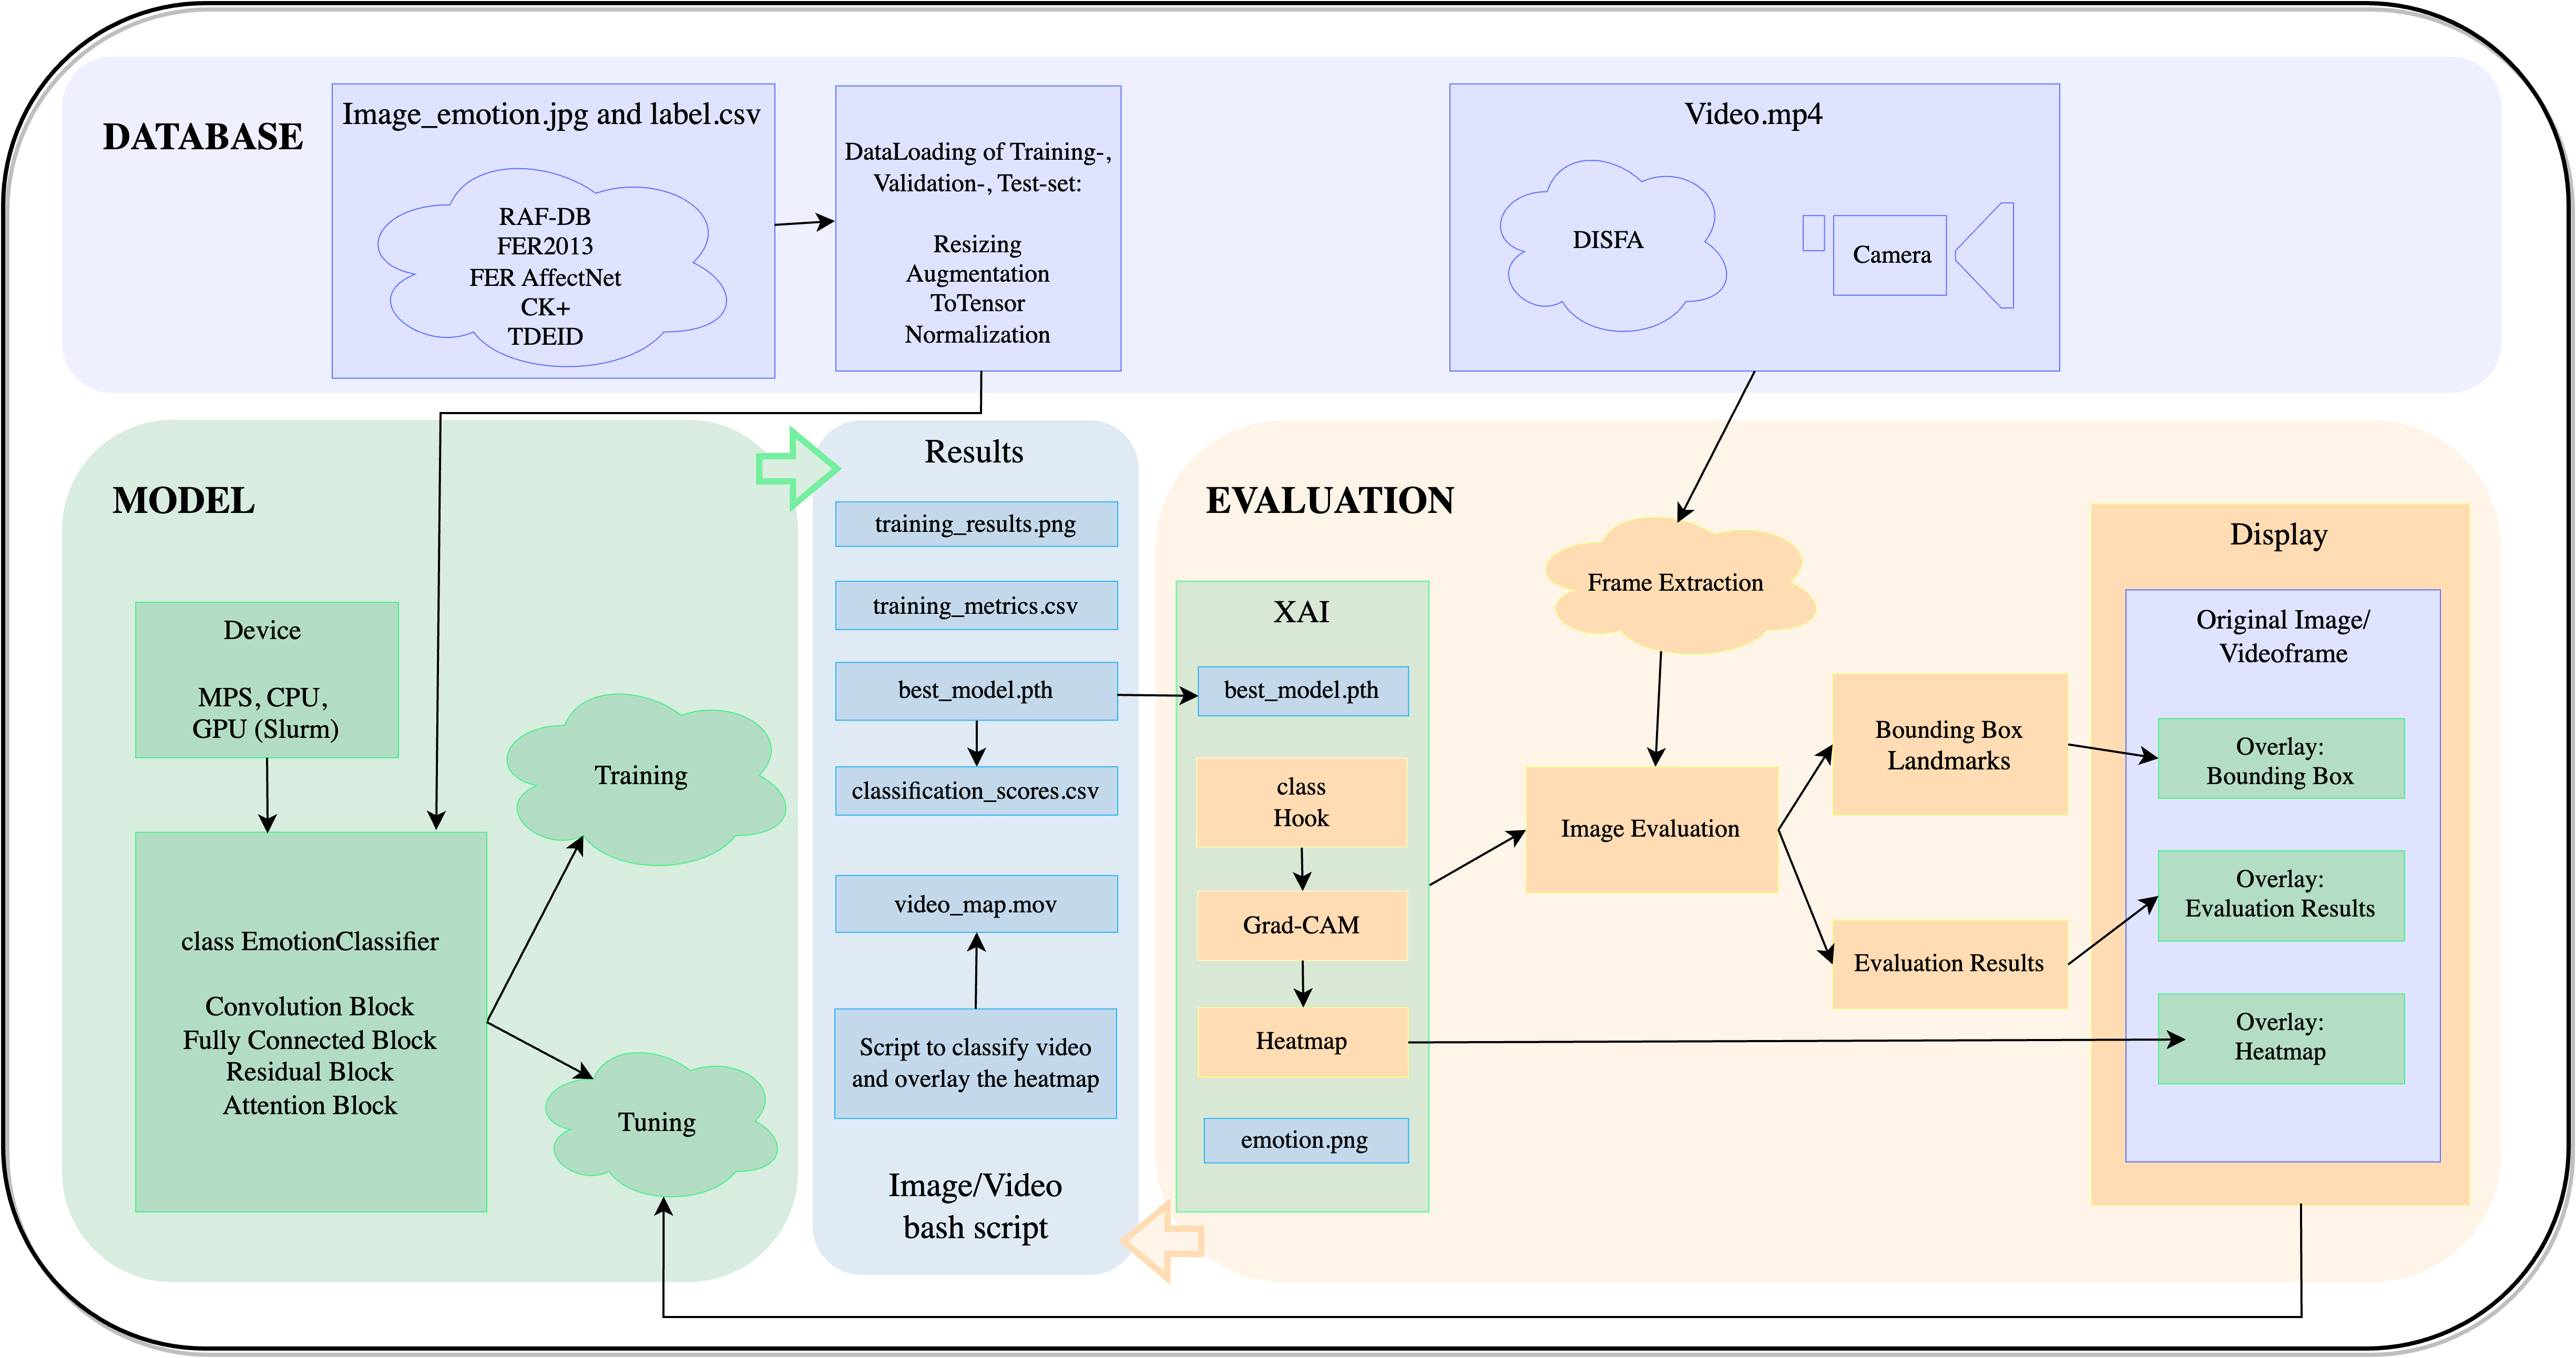
\includegraphics[width=\linewidth]{pipeline.png}
   \caption{Overview of the experimental pipeline.} 
   \label{fig:pipeline}
\end{figure*}

% add demo: see https://github.com/werywjw/SEP-CVDL/blob/main/paper/Selvaraju_Cogswell_Grad-CAM.pdf
\section{Related Work}
\label{sec:related}

\paragraph{Interpretable Emotion Classification.}

\citet{YinTLS019} focus on a specific area of interpretable visual recognition by learning from data a structured facial representation. 
\citet{Malik0R21} 

% TODO: add video related work (new paragraph)
\paragraph{Explainable AI (XAI).}
To understand the decision-making process of our model, 
we aim to explain our model in a more transparent and interpretable way using the Grad-CAM, 
i.e., Gradient-weighted CAM~\cite{SelvarajuCDVPB17}, 
a technique that is easier to implement with different architectures. 

Generally speaking, 
Class Activation Mapping (CAM)~\cite{ZhouKLOT16} is a technique popularly used in CNNs to visualize and understand the regions of an input image that contribute the most to a particular class prediction. 
CAM helps interpret CNN decisions by providing visual cues about the regions that influenced the classification, 
as it highlights the important regions of an image or a video, 
aiding in the understanding of the behavior of the model, 
which is especially useful for model debugging and further improvement. 
Typically,
CAM is applied to the final convolutional layer of a CNN. 
Besides proposing a method to visualize the discriminative regions of a CNN trained for the classification task, 
we adopt this approach from \citet{ZhouKLOT16} to localize objects without providing the model with any bounding box annotations. 
The model can therefore learn the classification task with class labels and is then able to localize the object of a specific class in an image or video. 

%~\footnote{~\url{https://medium.com/@stepanulyanin/implementing-grad-cam-in-pytorch-ea0937c31e82}}
% The weights connecting the feature maps to the output class are obtained.
% The weighted combination of feature maps, 
% representing the importance of each spatial location, is used to generate the CAM heatmap.
Despite CAM can provide valuable insights into the decision-making process of deep learning models, 
especially CNNs, 
CAM must be implemented in the last layer of a CNN or before the fully connected layer.

\citet{chattopadhay2018grad} proposed Grad-CAM++,

\section{Experimental Setup}
\label{sec:setup}

All the experiments are implemented in Python. 
We also use Shell and Jupyter Notebook for generating image and video scripts. 
The experiment and evaluation are conducted on two MacBook Pros 
(M1 Pro-Chip with 10-core CPU and 16-core GPU; Intel Core i9 with 2.3 GHz 8-Core). 

\subsection{Dataset}
\label{sec:setup:datasets}

% https://www.mdpi.com/1424-8220/22/21/8089

\begin{table*}[ht]
  \centering
  \resizebox{.99\textwidth}{!}{
  \begin{tabular}{@{}lrcccccc|c@{}}
      \toprule
      \textsc{Dataset} & \textsc{Split} & \# happiness & \# surprise & \# sadness & \# anger & \# disgust & \# fear & \# total videos/images \\
      \midrule
      DISFA~\cite{MavadatiMBTC13} & Test &  &  &  &  &  &  & 27 \\ % TODO Leah
      \midrule
      \multirow{2}{*}{RAF-DB~\cite{li_reliable_2017,li2019reliable}} & Train & 4772 & 1290 & 1982 & 705 & 717 & 281 & 9747 \\
      &Test &1185&329&478&162&160&74& 2388 \\
      \midrule
      \multirow{2}{*}{FER2013~\cite{BarsoumZCZ16}} & Train & 7215 & 3171 & 4830 & 3994 & 436 & 4097 & 23743 \\
      &Test &1774&831&1247&958&111&1024& 5945 \\
      \midrule
      FER AffectNet~\cite{Mollah2019ANet} & Train & 3091 & 4039 & 5044 & 3218 & 2477 & 3176 & 21045 \\
      \midrule
      CK+~\cite{LuceyCKSAM10} & Train & 69 & 83 & 28 & 45 & 59 & 25 & 309 \\
      \midrule
      TFEID~\cite{tfeid,LiGL22} & Train & 40 & 36 & 39 & 34 & 40 & 40 & 229 \\
      \midrule
      \midrule
      \multirow{3}{*}{FER \textsc{GiMeFive}} & Train  & 15187 & 8619 & 11923 & 7996 & 3729 & 7619 & \textbf{55073} \\
      & Test & 2959 & 1160 & 1725 & 1120 & 271 & 1098 & \textbf{8333} \\
      & Valid & 100 & 100 & 100 & 100 & 100 & 100 & \textbf{600} \\ 
      \bottomrule
  \end{tabular}
  }
\caption{Overview of the data statistics for each emotion class and the total number of videos/images in our experiment.}
\label{tab:data}
\end{table*}

To initiate the project, 
we gathered image databases representing different types of emotional expressions from 
\textit{Real-world Affective Faces Database} (RAF-DB, in-the-wild expression)~\cite{li_reliable_2017,li2019reliable}, 
\textit{Facial Expression Recognition} 2013 (FER2013, real-time wild expression)~\cite{BarsoumZCZ16}, 
\textit{Facial Expression Recognition AffectNet Database} (FER AffectNet, in-the-wild expression)~\cite{Mollah2019ANet}, 
\textit{Extended Cohn-Kanade Dataset Plus} (CK+, posed expressions)~\cite{LuceyCKSAM10}, 
and \textit{Taiwanese Facial Expression Image Database} (TFEID, posed expressions)~\cite{tfeid,LiGL22}.
These image datasets come in folder-structure classification (See \Cref{tab:data} 
for statistic details with specific numbers on training, test, and validation set for each emotion class). 

For reviewing explainable AI, 
we used the video dataset \textit{Denver Intensity of Spontaneous Facial Action Database} 
(DISFA, spontaneous expressions)~\cite{MavadatiMBTC13}, 
which comprises two sets of videos, 
differentiated by capturing various camera angles. 
Each set consists of 27 videos, with each video comprising 4844 frames, 
resulting in 130788 images for each camera angle and a total of 261576 images across both angles. 
% which contains a variety of levels of intensity in expression. 

\paragraph{Image Preprocessing.}
The procedure is proceeded from public institutions and kaggle~\cite{kaggle_rafdb,kagaff}. 
To enhance the generalizability and robustness of our model, 
we aggregate these five FER image benchmarks into a new customized dataset called FER 
\textsc{GiMeFive}~\footnote{\url{https://github.com/werywjw/data}}. 
More specifically, 
the training set of FER \textsc{GiMeFive} is aggregated from the training sets of the five image datasets (55073 images in total), 
while the test set is combined from the test sets of RAF-DB and FER2013 (8333 images). 
The validation set is given with equal 100 images per class to test the performance of models. 

Building upon these image databases, we exclusively analyze human faces representing 6 emotions. 
That is, we first generalize a folder structure and append the emotion labels 0 to 5 to the name of each matching image 
(0 for happiness, 1 for surprise, 2 for sadness, 3 for anger, 4 for disgust, and 5 for fear).
For implementation, 
we create a script for generating CSV files to store all the image names and their corresponding labels to later efficiently pass to the model. 
The images together with the CSV file are loaded and preprocessed for training. 
Therefore, we manipulate the pixel data through resizing, 
augmentation, conversion to grayscale, and create tensors and normalization. 
The images are converted to greyscale with three channels at $64 \times 64$ resolution in the JPG format, 
as our original CNN is designed to work with three-channel inputs. 
Typically, we assume that the color of the image does not affect the emotion classification. 

\paragraph{Video Preprocessing.}
For testing our model, we establish standards for extracted frames from videos or live webcam streams. 
Each frame, extracted for testing, undergoes scanning for the region of interest, the face(s). 
To achieve this, 
we implement the \texttt{CascadeClassifier}~\cite{casc_class} incorporating the Viola-Jones algorithm introduced by \citet{990517} to power, 
in our case, face detection, 
since the Viola-Jones algorithm revolutionizes real-time object detection. 

As part of the video preprocessing, 
we run every frame through the \texttt{FaceClassifier} to detect our region of interest, 
and crop the rectangle region. 
The cropped image is then also preprocessed by resizing to $64 \times 64$ resolution, 
then converted to greyscale with three channels, 
after that, a tensor is generated and then normalized. 
Every cropped image is evaluated through our model so that the classification can be further used for interpretation. 

\subsection{Model Architecture}
\label{sec:setup:model}

In order to compare the performance of our \textsc{GiMeFive} with other models, 
we replicate several state-of-the-art CNNs from scratch, 
which include \textit{Visual Geometry Group} (VGG)~\cite{SimonyanZ14a} and 
ResNet~\cite{HeZRS16} on two FER benchmarks (i.e., RAF-DB and FER 2013), 
as well as FER \textsc{GiMeFive} (see \Cref{sec:setup:datasets} for details). 

\tikzstyle{block} = [rectangle, draw, fill=LMUGreen!30, text width=5em, text centered, rounded corners, minimum height=4em]
\tikzstyle{line} = [draw, -latex', line width=0.7pt]

\begin{figure*}[ht]
  \centering
  \resizebox{.99\textwidth}{!}{
  \begin{tikzpicture}[node distance=2.7cm, auto]
      \node [block] (input) {Input Layer};
      \node [block, right of=input] (conv1) {Conv Block 1 \\ 64 Filters};
      \node [block, right of=conv1] (conv2) {Conv Block 2 \\ 128 Filters};
      \node [block, right of=conv2] (conv3) {Conv Block 3 \\ 256 Filters};
      \node [block, right of=conv3] (conv4) {Conv Block 4 \\ 512 Filters};
      \node [block, right of=conv4] (conv5) {Conv Block 5 \\ 1024 Filters};
      \node [block, right of=conv5] (adaptivePool) {Adaptive Avg Pool};
      \node [block, right of=adaptivePool] (fc) {Fully Connected Block};
      \node [block, right of=fc] (softmax) {Softmax Layer};

      \path [line] (input) -- (conv1);
      \path [line] (conv1) -- (conv2);
      \path [line] (conv2) -- (conv3);
      \path [line] (conv3) -- (conv4);
      \path [line] (conv4) -- (conv5);
      \path [line] (conv5) -- (adaptivePool);
      \path [line] (adaptivePool) -- (fc);
      \path [line] (fc) -- (softmax);
  \end{tikzpicture}
  }
  \caption{Overview of the \textsc{GiMeFive} model architecture 
  (see \Cref{fig:modeldetail} for a detailed version).} 
  \label{fig:model}
\end{figure*}

\paragraph{VGG16.}
\citet{SimonyanZ14a} developed the VGG16 model, 
which represents

\paragraph{ResNet.}
In principle, 
deeper neural networks with more parameters are more difficult to train. 
Inspired by \citet{HeZRS16}, 
we implement the ResNet18 and ResNet34 with the residual block to ease the training process. 

\paragraph{\textsc{GiMeFive}.}
Our model architecture is illustrated in \Cref{fig:model} (see \Cref{fig:modeldetail} for details). 
The input of our emotion recognition model is an image with 3 channels at $64 \times 64 $ resolution. 
The output is 6 emotion classes. % : happiness, surprise, sadness, anger, disgust, and fear. 
We implement an emotion classification model from scratch with four convolution blocks as our baseline at the very beginning. 
Despite the larger kernel being able to provide more information and a wider area view due to more parameters, 
we use a $3 \times 3$ kernel size for all convolutional layers, 
as it is efficient to train and share the weights without expensive computation. 
Following each convolutional layer, 
batch normalization is used for stabilizing the learning by normalizing the input to each layer. 
Meanwhile, 
BN ensures forward propagated signals to have non-zero variances. 
We interleaved with the max pooling layer because it reduces the spatial dimensions of the input volume. 
Afterward, three linear layers are applied to extract features to the final output. 
We also add a 50\% dropout layer between the first and second linear layers to prevent overfitting. 
Verified by \citet{BarsoumZCZ16}, 
the dropout layers are effective in avoiding model overfitting. 
The activation function after each layer is \textit{Rectified Linear Unit} (ReLU), 
since it introduces the non-linearity into the model, 
allowing it to learn more complex patterns. 
Our best model \textsc{GiMeFive} is later optimized with the dropout rate at 20\% after the max pooling layer as well.

\section{Evaluation}
\label{sec:evaluation}

For evaluation, we use the metric accuracy to see if our model can classify the facial emotions correctly. 
We report all the training, testing, and validation accuracies in 
\% to compare the performance of our \textsc{GiMeFive} with other state-of-the-art methods. 

The loss function employed for all models is cross-entropy (CE), 
which is typically for multi-class classification. 
Mathematically, the CE loss is defined as follows: 
\begin{equation}
  \mathcal{L}_{\text{CE}} = -\sum_{i=1}^{n} y_i \log(p_i),
\end{equation}
where $y_i$ is the true label and $p_i$ is the predicted probability of the $i$-th class. 
Here $n$ denotes the total number of classes, in our case, 6.

\subsection{Evaluation Results}
\label{sec:evaluation:results}

\begin{table*}[ht]
  \centering
  % \resizebox{.99\textwidth}{!}{
  \begin{tabular}{@{}llcccccr@{}}
    \toprule 
    \multirow{2}{*}{\textsc{Dataset}}&\multirow{2}{*}{\textsc{Models}}&\multirow{2}{*}{\textsc{\# Layers}}&\multirow{2}{*}{\textsc{Architecture}} & \multicolumn{3}{c}{\textsc{Accuracies}} & \multirow{2}{*}{\textsc{\# Parameters}} \\
    \cline{5-7}
    &&&& Train & Test & Valid  &  \\
    \midrule
    \multirow{9}{*}{RAF-DB~\cite{li_reliable_2017,li2019reliable}} &VGG16~\cite{SimonyanZ14a} & 16 &+BN&93.8&83.3&68.8&72460742\\ 
    & ResNet18~\cite{HeZRS16} & 18 & +RB  & 98.9 & 81.3 & 67.9 & 11179590 \\
    & ResNet34~\cite{HeZRS16} & 34 & +RB  & \textbf{100.0} & 83.7 & 72.0 & 21287750 \\
    &\textsc{GiMeFive} (Baseline) & 13 & +BN-SE & 96.6 & 80.6 & 66.8 & 2606086 \\ 
    &\textsc{GiMeFive} (Ours) & 10 & -BN-SE & 96.3 & 76.9 & 60.6 & 10474118 \\
    &\textsc{GiMeFive} (Ours) & 16 & +BN+SE & 98.4 & 81.7 & 71.1 & 10478598 \\
    &\textsc{GiMeFive} (Ours) & 15 & +BN-SE & 98.6 & 83.1 & 72.1 & 10478086 \\
    &\textsc{GiMeFive} (Ours)\textcolor{LMUGreen}{$^\star$} & 15 & +DO+BN-SE & 97.0 & \textbf{86.5} & \textbf{78.1} & 10478086 \\
    &\textsc{GiMeFive} (Ours) & 17 & +BN-SE & 97.5 & 82.5 & 70.0 & 41950726 \\ 
    \midrule
    \multirow{7}{*}{FER2013~\cite{BarsoumZCZ16}} & VGG16~\cite{SimonyanZ14a} & 16 & +BN & 69.0 & 49.4 & 35.6 & 72460742 \\
    & ResNet18~\cite{HeZRS16} & 18 & +RB  & 92.6 & 64.7 & 42.1 & 11179590 \\
    & ResNet34~\cite{HeZRS16} & 34 & +RB  & \textbf{97.6} & 67.1 & 43.6 & 21287750 \\
    & \textsc{GiMeFive} (Baseline) & 13 & +BN-SE & 86.6 & 64.1 & 40.2 & 2606086 \\
    &\textsc{GiMeFive} (Ours) & 15 & +BN-SE & 89.6 & 65.6 & 40.7 & 10478086 \\
    &\textsc{GiMeFive} (Ours)\textcolor{LMUGreen}{$^\star$} & 15 & +DO+BN-SE & 69.7 & \textbf{67.5} & \textbf{46.2} & 10478086 \\
    &\textsc{GiMeFive} (Ours) & 17 & +BN-SE & 96.0 & 65.5 & 41.6 & 41950726 \\
    \midrule
    \midrule
    \multirow{5}{*}{FER \textsc{GiMeFive}} & VGG16~\cite{SimonyanZ14a} & 16 & +BN & 79.4 & 53.7 & 61.4 & 72460742 \\
    & ResNet18~\cite{HeZRS16} & 18 & +RB  & \textbf{96.5} & 72.4 & 73.8 & 11179590 \\
    & ResNet34~\cite{HeZRS16} & 34 & +RB  & 94.5 & 70.8 & 72.8 & 21287750 \\
    &\textsc{GiMeFive} (Ours)\textcolor{LMUGreen}{$^\star$} & 15 & +DO+BN-SE & 84.9 & \textbf{75.3} & \textbf{75.0} & 10478086 \\
    &\textsc{GiMeFive} (Ours) & - & +BN+SE+RB & 95.2 & 70.4 & 74.5 & 95051014 \\
    \bottomrule
  \end{tabular}
  % }
  \caption{Accuracies (\%) for different models with specific architectures and numbers of parameters and layers in our experiments 
  (Note that \textcolor{LMUGreen}{$^\star$} denotes our best GiMeFive; 
  BN stands for the batch normalization, 
  RB for residual block, 
  SE for the squeeze and excitation block, 
  and DO for dropout; 
  +/- represent with/without respectively). 
  The confusion matrix of the validation set in terms of the number of classified images is shown in \Cref{fig:matval}, 
  while the result of the test set on the RAF-DB is given in \Cref{fig:mattest}.} 
  \label{tab:model}
\end{table*}

As seen in \Cref{tab:model}, 
the test results are aggregated from the database RAF-DB~\cite{kaggle_rafdb} and FER2013~\cite{kaggle_fer}.
Different combinations of functions from the \texttt{pytorch.transforms} library are tested for augmentation from those already established filters. 

Our CNN without random augmentation outperforms the other models in terms of accuracy, 
indicating that this kind of augmentation is not able to help our model predict the correct label, 
thus we later aim to optimize with other augmentation techniques to capture more representative features of different emotions.
Further research is orientated on papers engaging similar investigations~\cite{ZeilerF14,li_reliable_2017,VermaMRMV23}.

Adding an extra convolutional block to the model with more parameters does not necessarily lead to better performance.
Batch normalization can indeed improve the performance of the model. 

% TODO (Jiawen)

\subsection{Interpretable Results}
\label{sec:evaluation:inter}

\begin{figure}[ht]
  \centering
   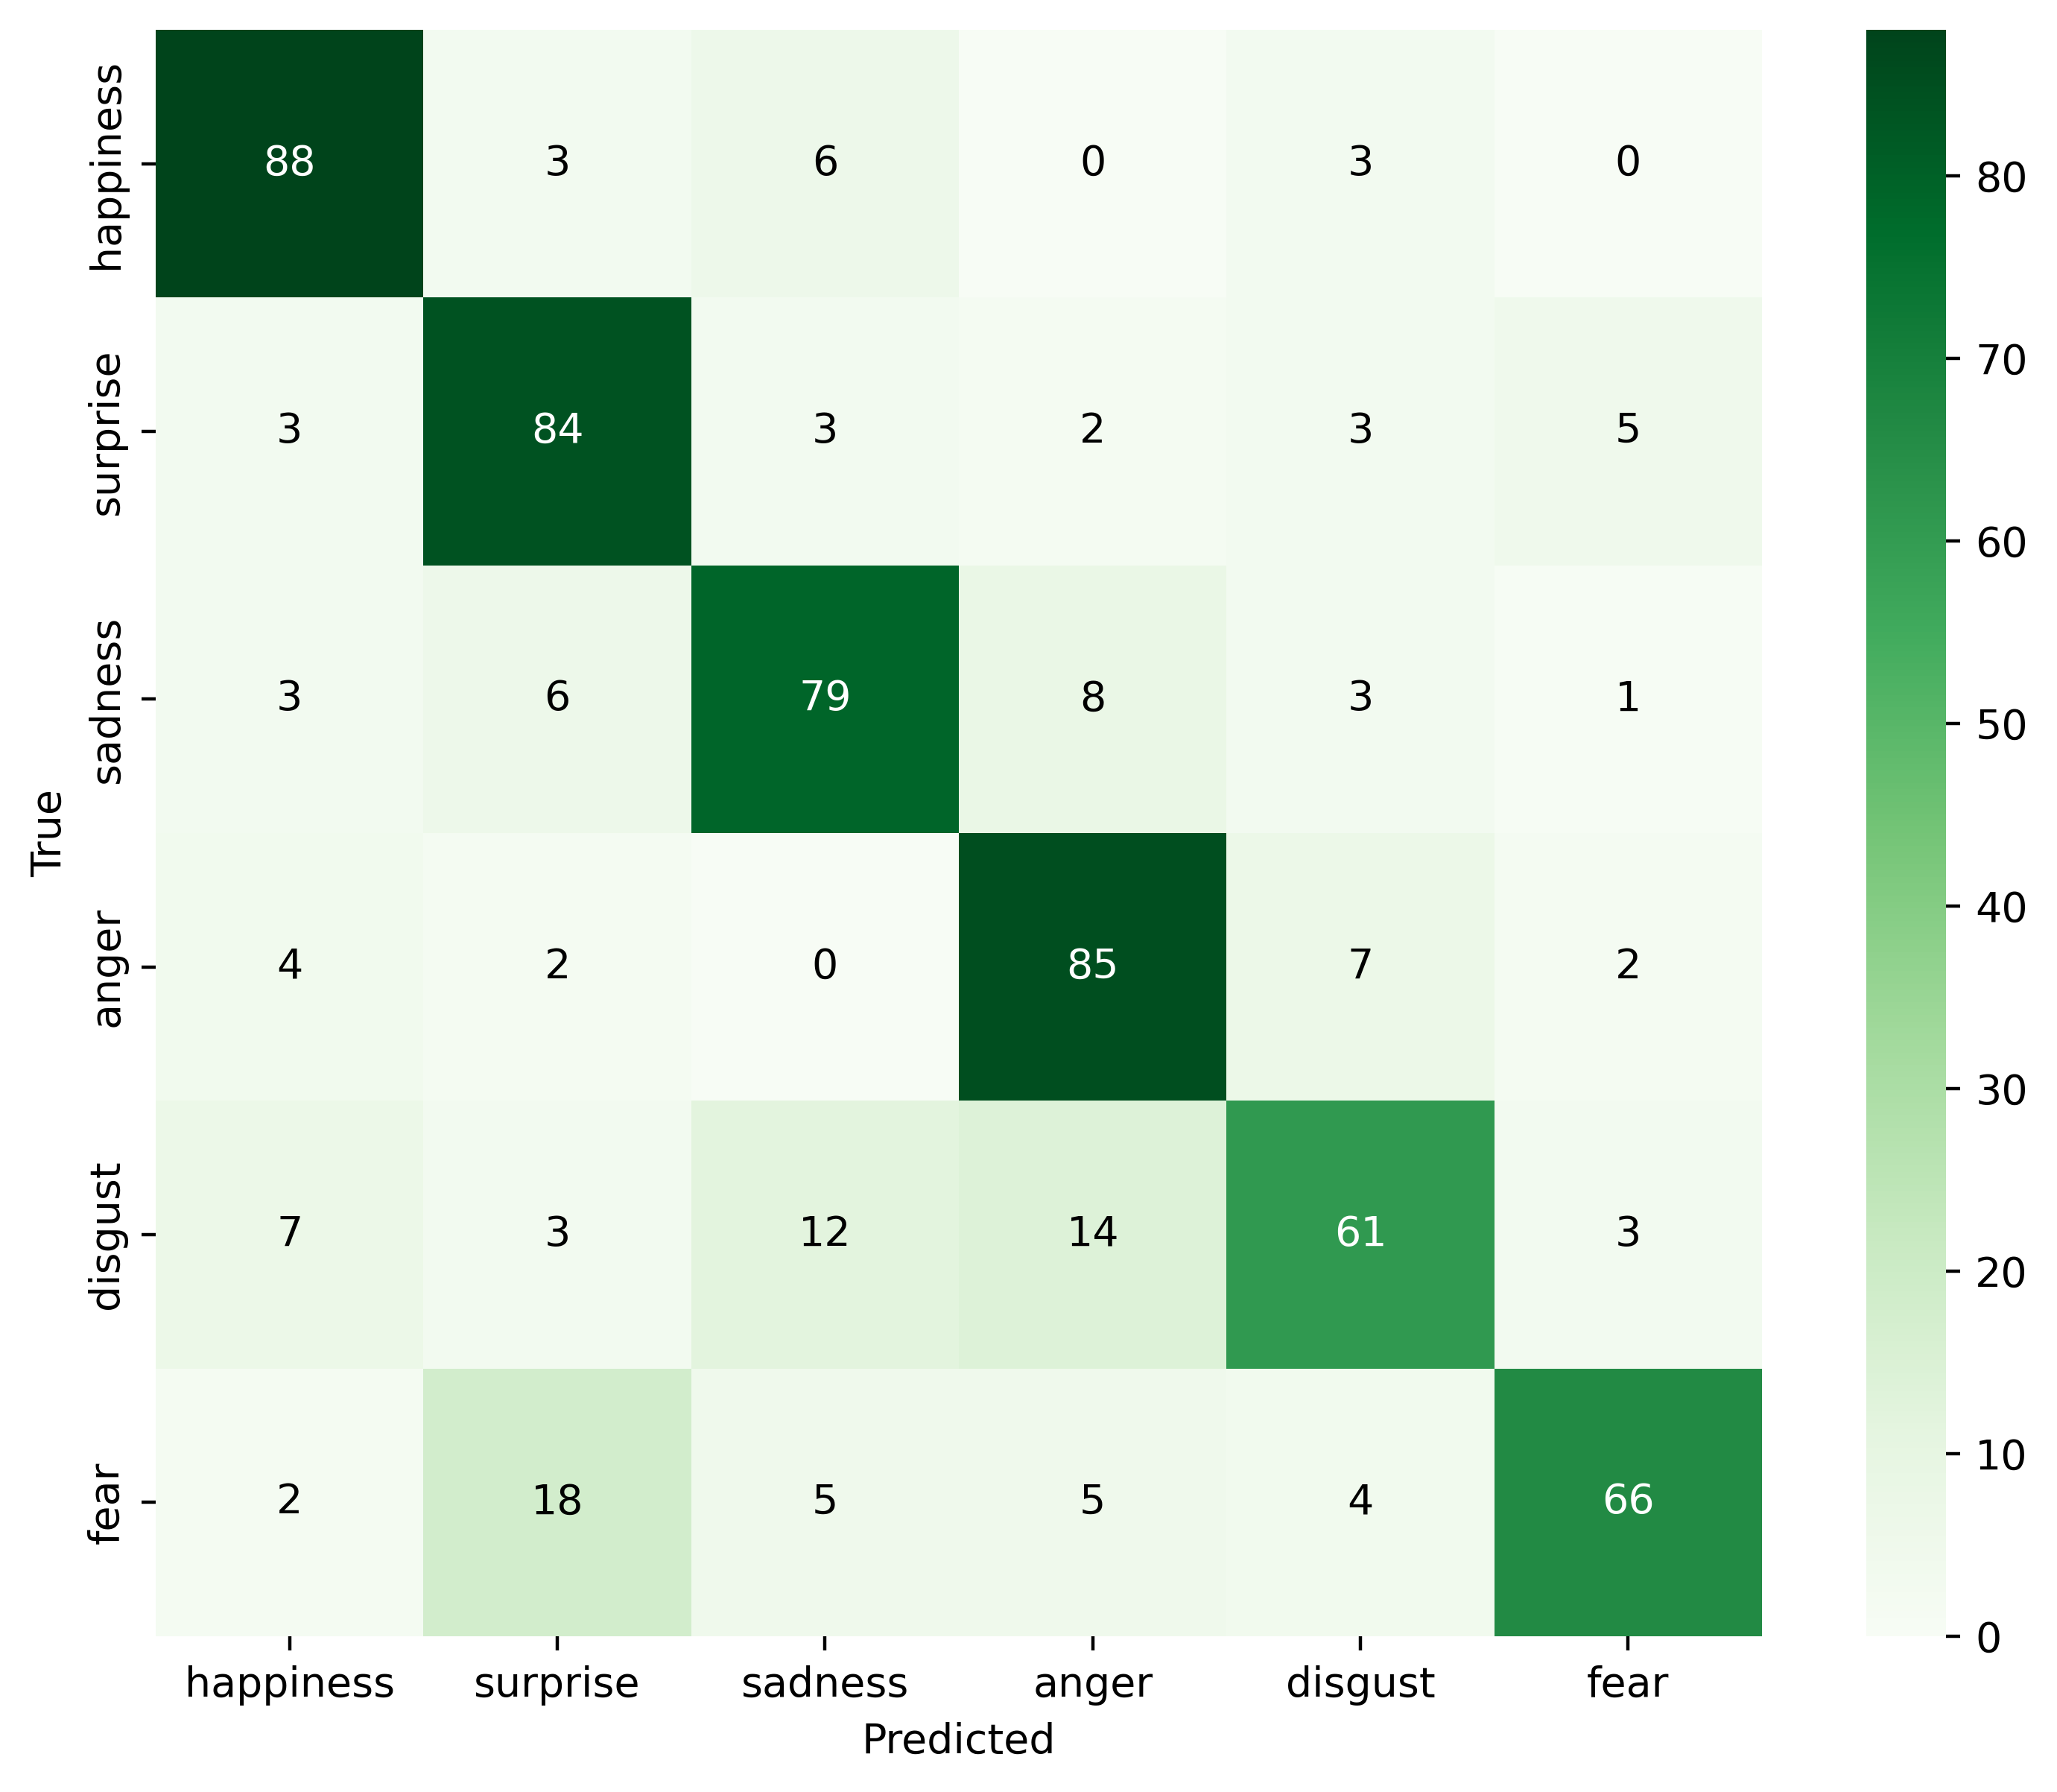
\includegraphics[width=\linewidth]{matval.png}
   \caption{Overview of the confusion matrix on the validation set.} 
   \label{fig:matval}
\end{figure}

\paragraph{Classification Scores.} 
To further analyze the individual scores of each class of the model, 
we write a script that takes a folder path as input and iterates through the images inside a subfolder to record the performance of our best model \textsc{GiMeFive}. 
This CSV file is represented with the corresponding classification scores via the softmax. 
Meanwhile, 
we also generate a confusion matrix heatmap to visualize the performance of the model with respect to each emotional class.

As shown in \Cref{fig:matval}, 
we observe that our \textsc{GiMeFive} can predict the happiness class with the highest accuracy, 
while the class with the lowest accuracy is disgust. 
This is understandable, 
as the facial emotions such as sadness and anger are similar to disgust, 
especially when humans sometimes also represent disgusting and angry emotions at the same time. 
Moreover, 
the confusion matrix illustrates that the model has good performances in terms of classifying surprise, sadness, and anger as well. 


\begin{figure}[ht]
  \centering
  \begin{subfigure}{0.3\linewidth}
    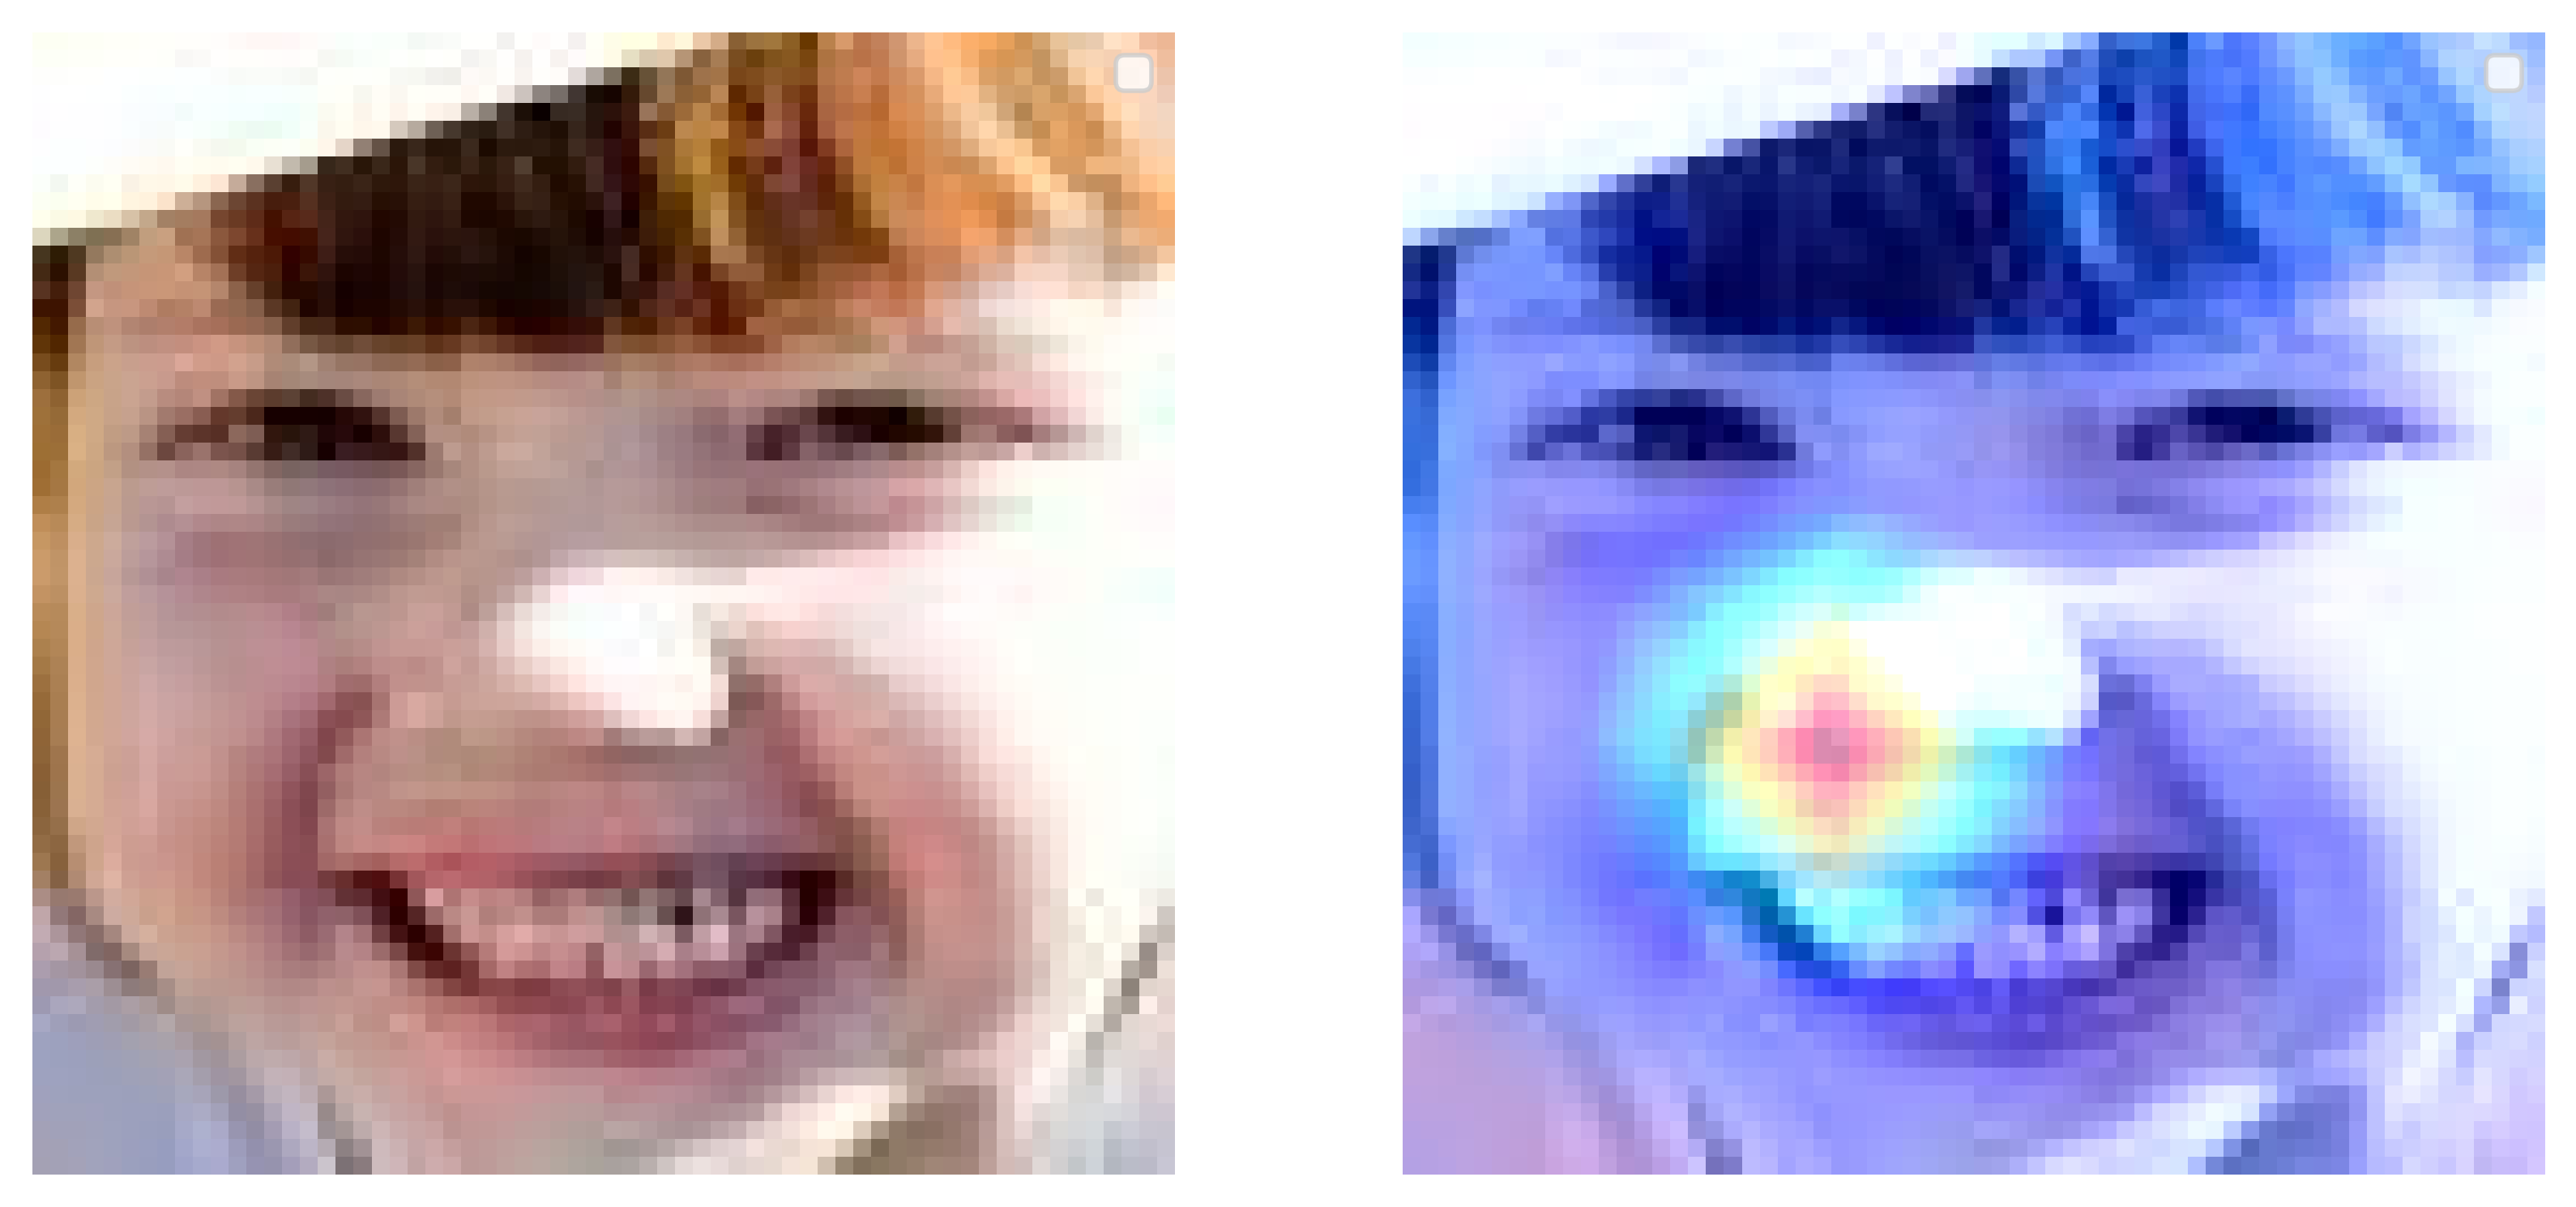
\includegraphics[width=\linewidth]{xai_happiness_.png}
    \caption{Happiness.}
    \label{fig:xai1}
  \end{subfigure}
  \hfill
  \begin{subfigure}{0.3\linewidth}
    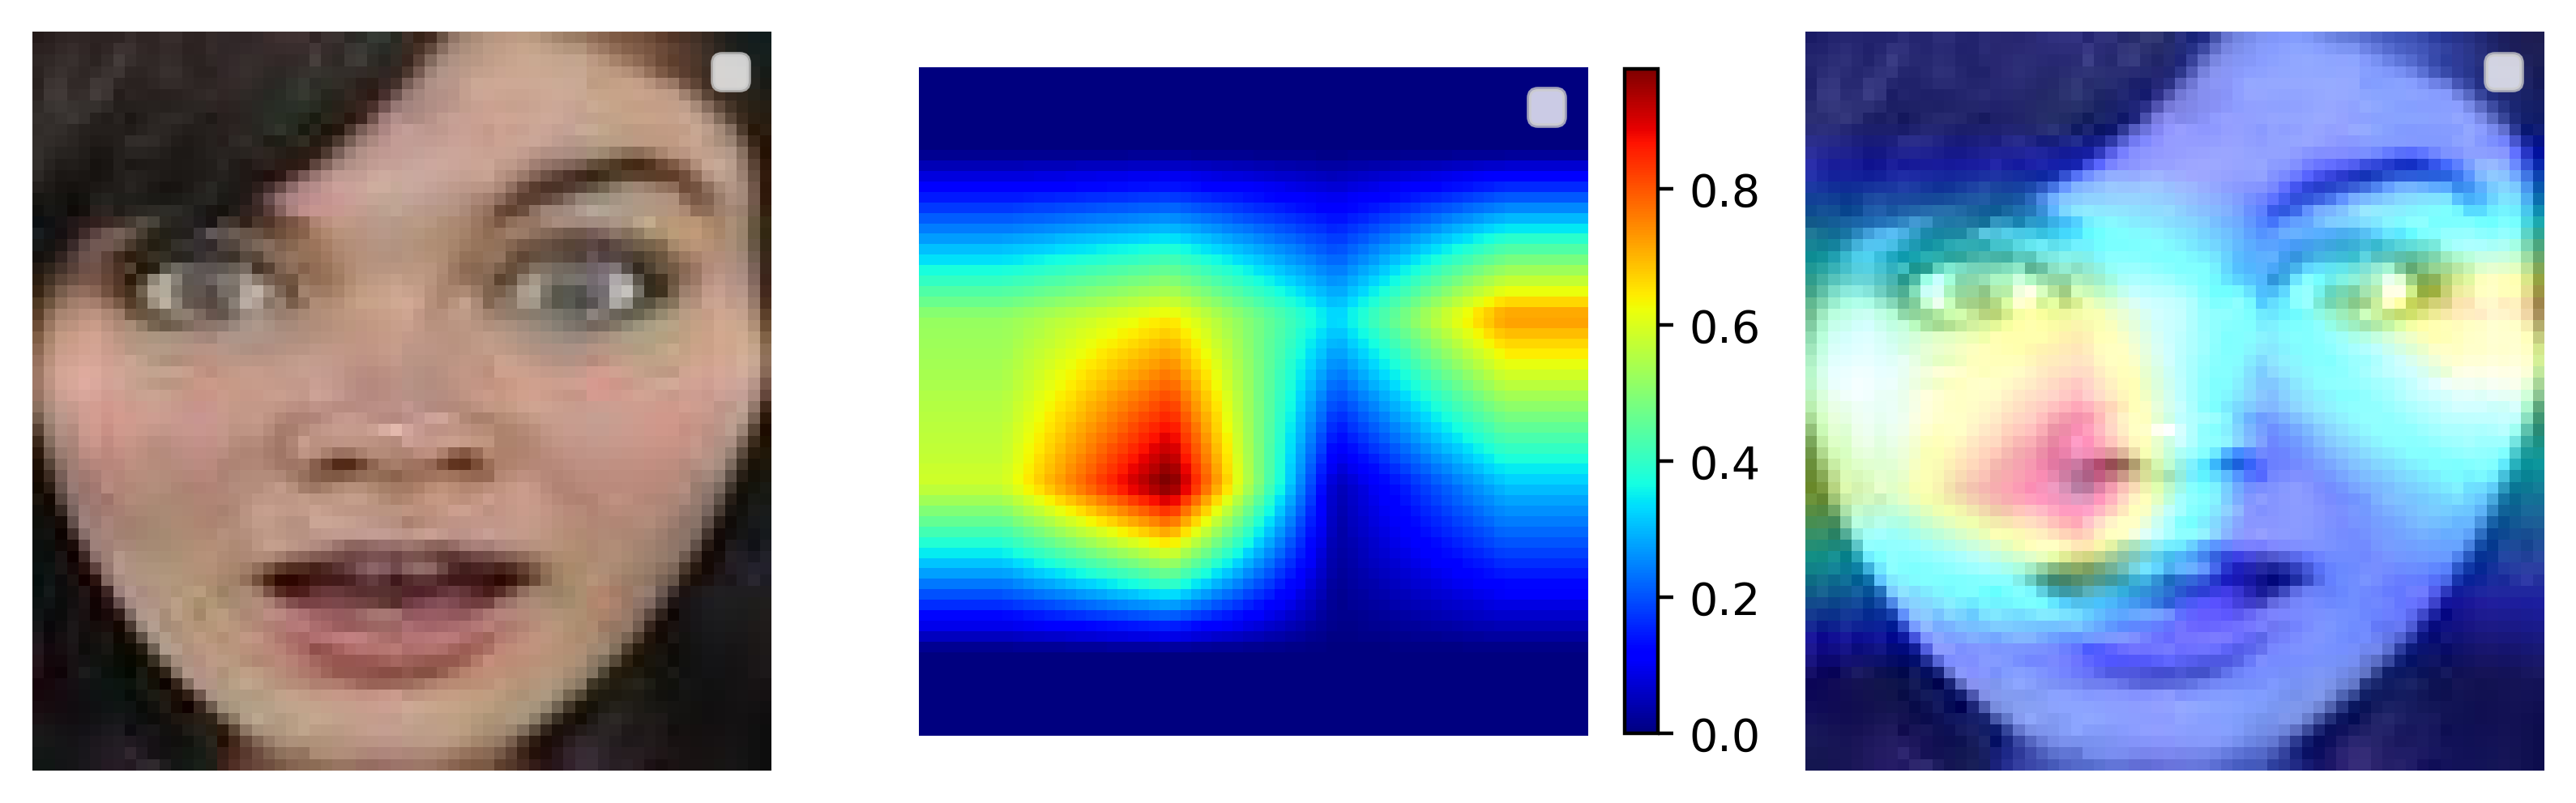
\includegraphics[width=\linewidth]{xai_surprise.png}
    \caption{Surprise.}
    \label{fig:xai2}
  \end{subfigure}
  \hfill
  \begin{subfigure}{0.3\linewidth}
    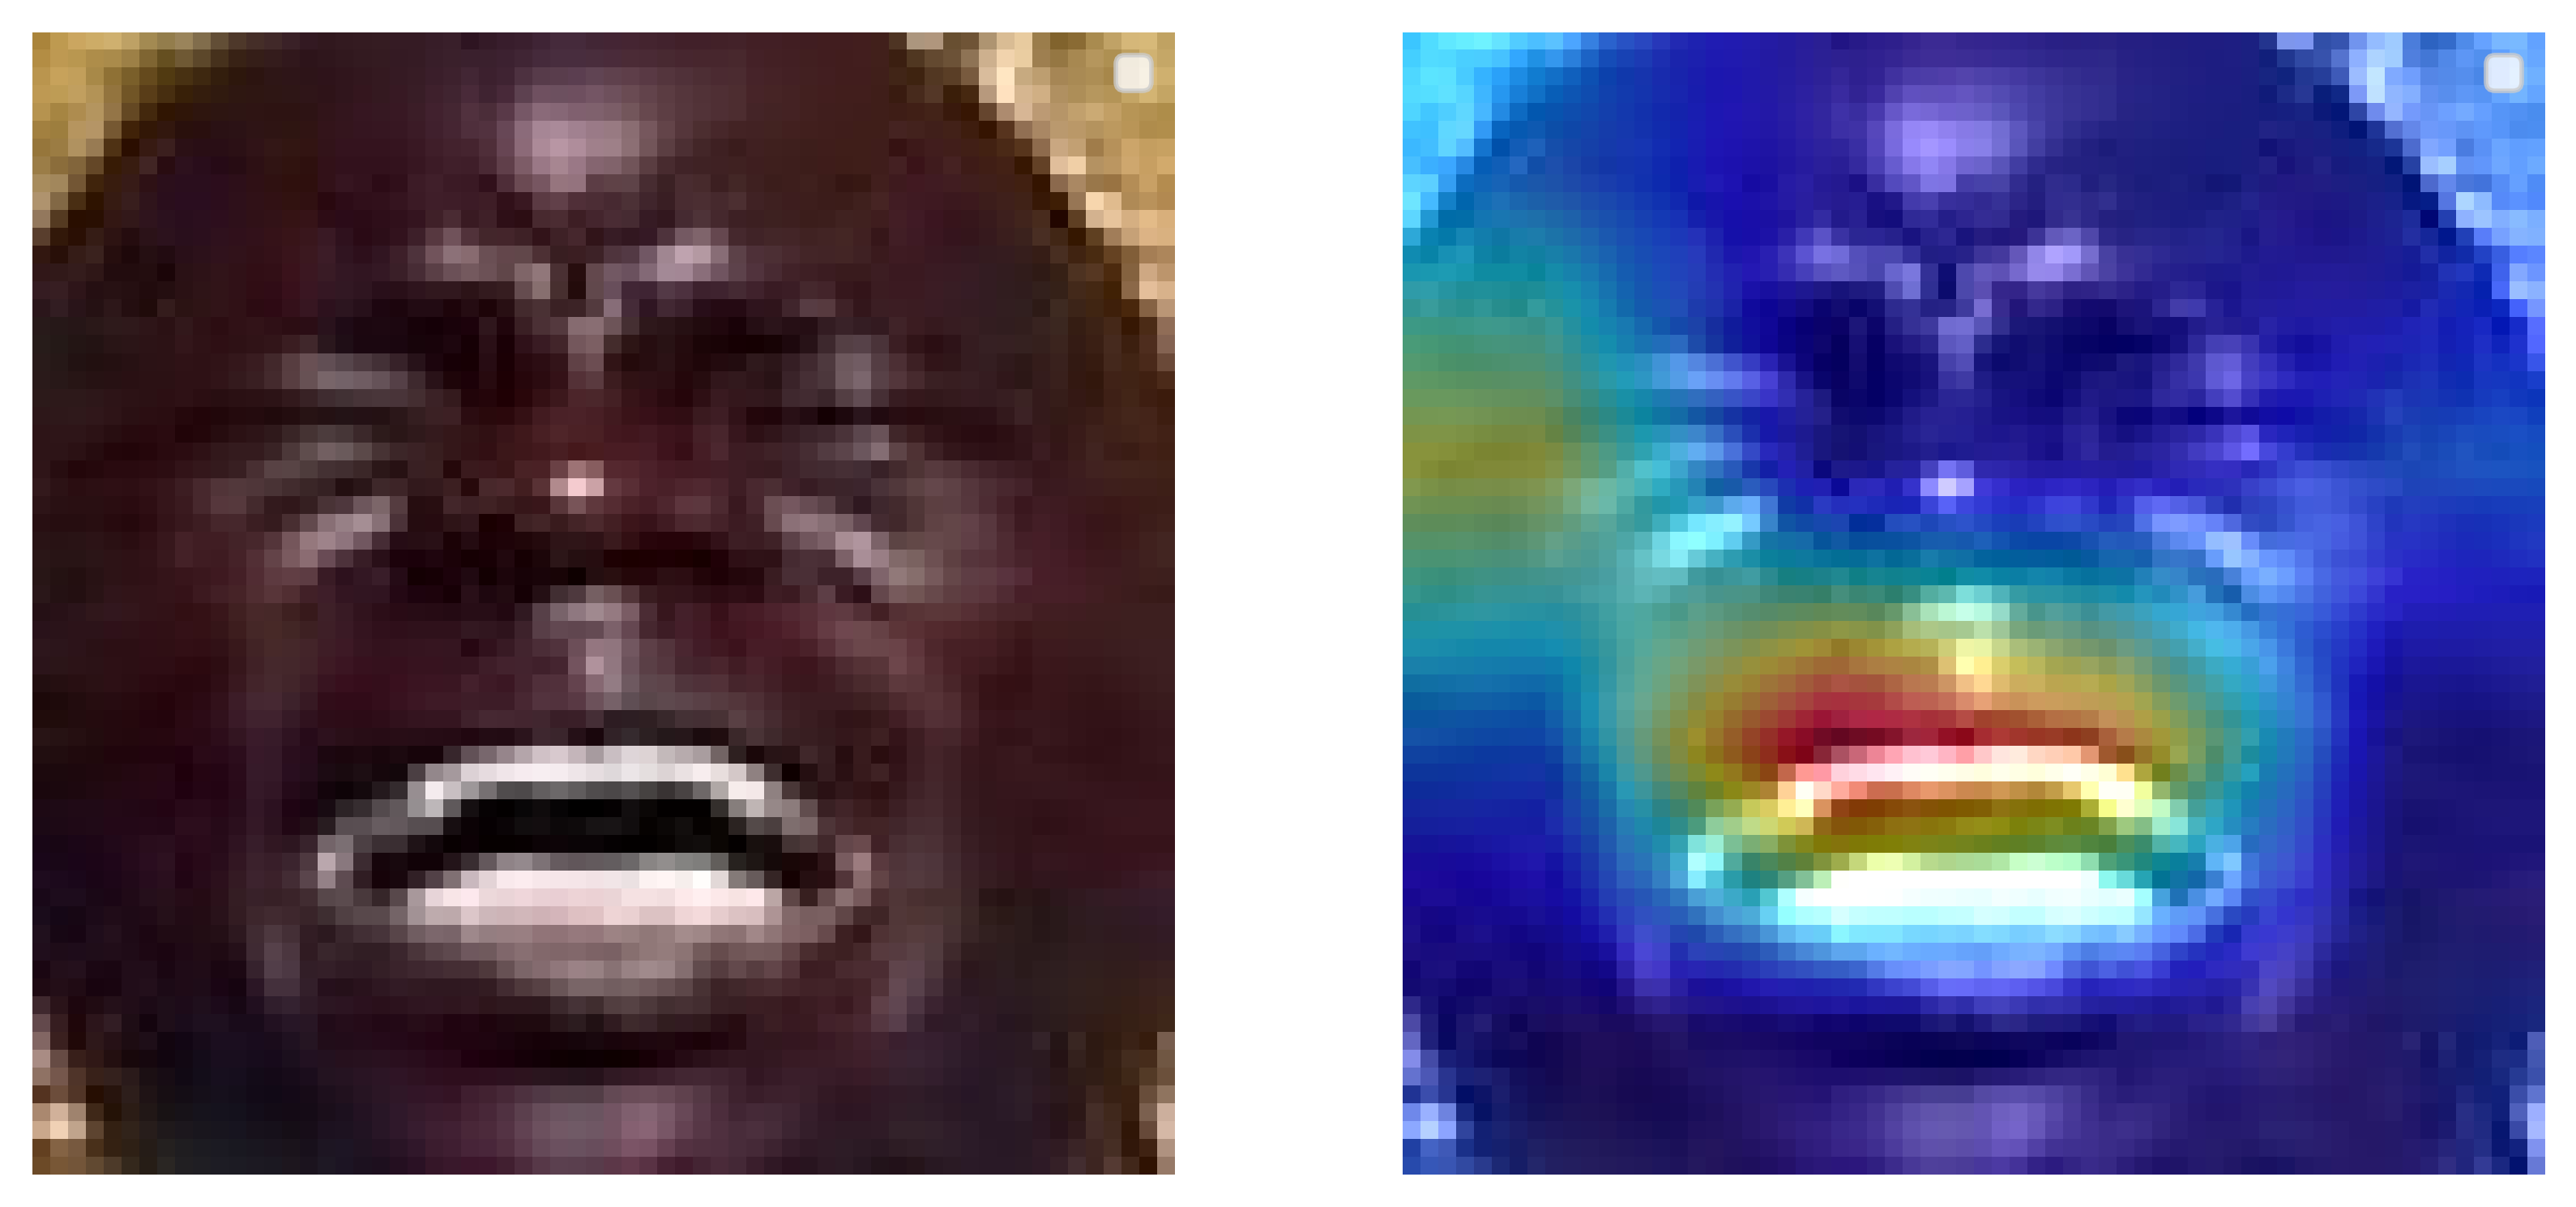
\includegraphics[width=\linewidth]{xai_sadness_.png}
    \caption{Sadness.}
    \label{fig:xai3}
  \end{subfigure}
  \hfill
  \begin{subfigure}{0.3\linewidth}
    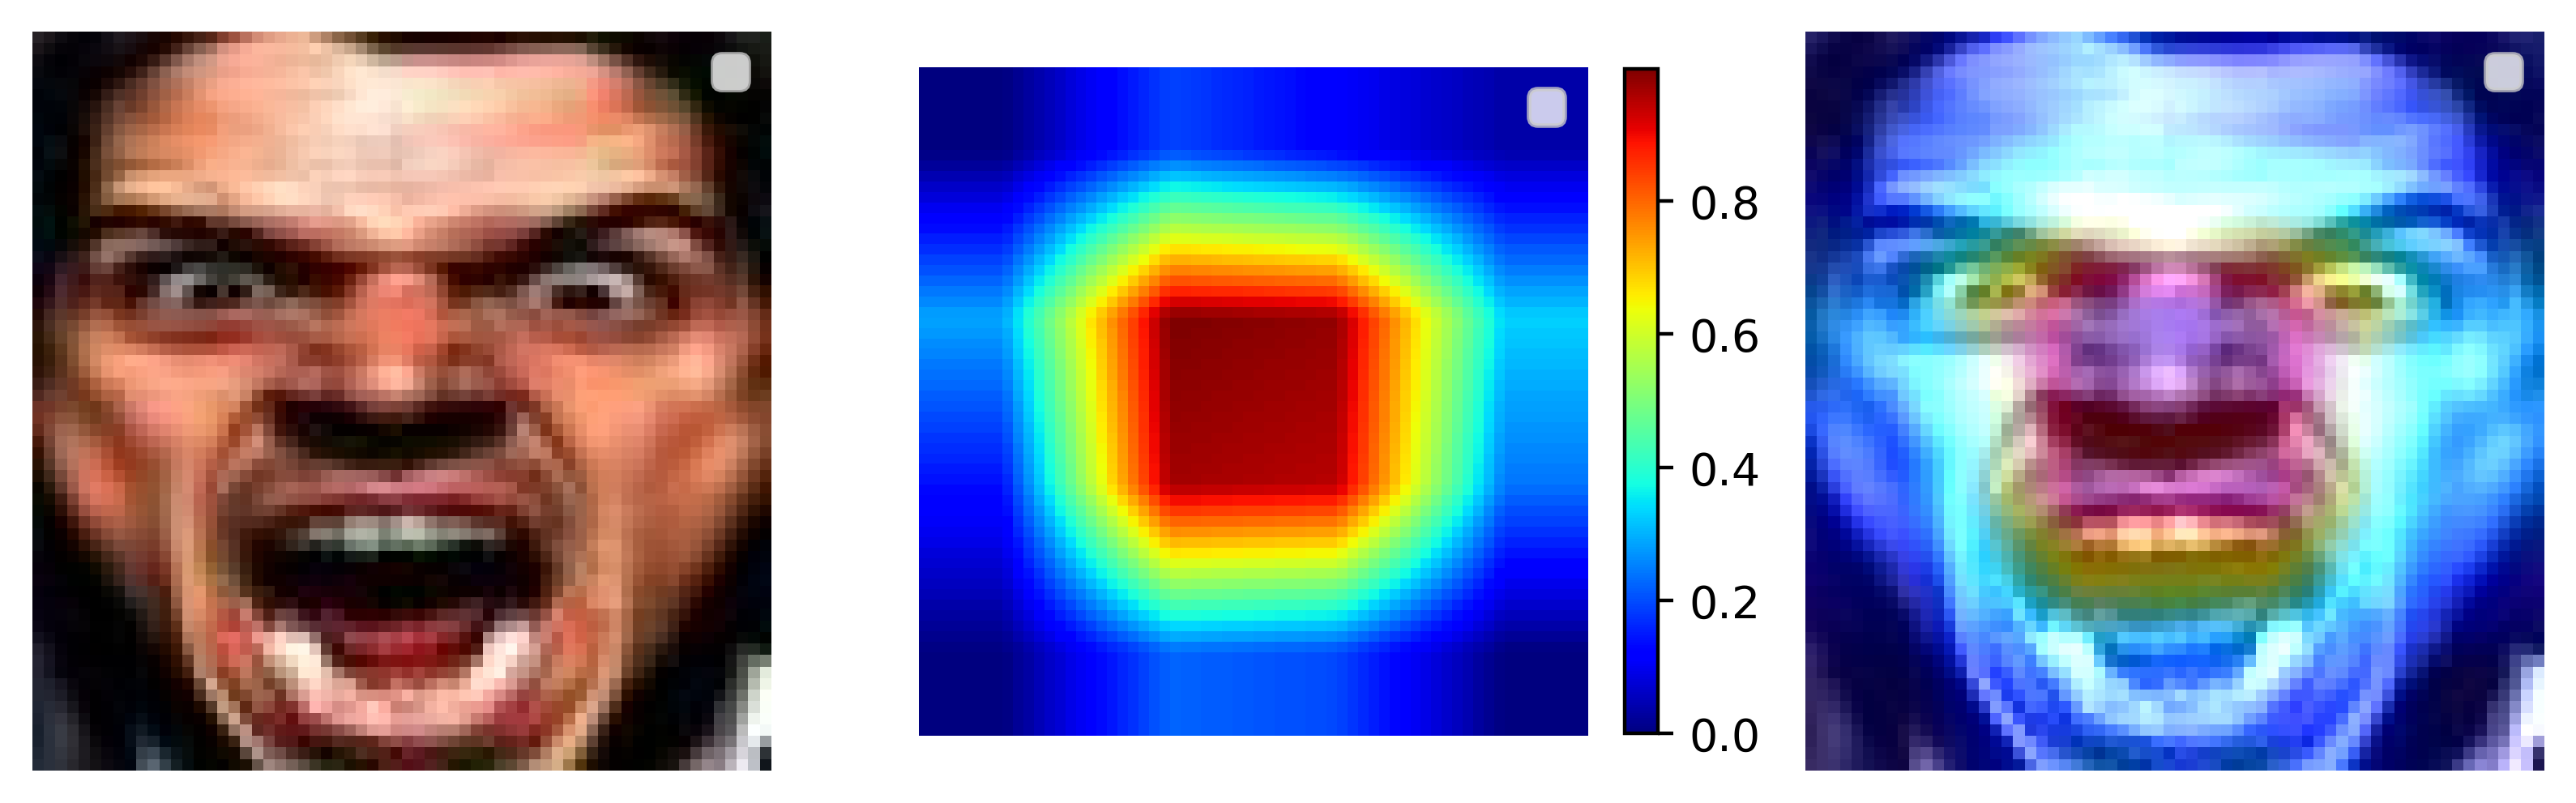
\includegraphics[width=\linewidth]{xai_anger.png}
    \caption{Anger.}
    \label{fig:xai4}
  \end{subfigure}
  \hfill
  \begin{subfigure}{0.3\linewidth}
    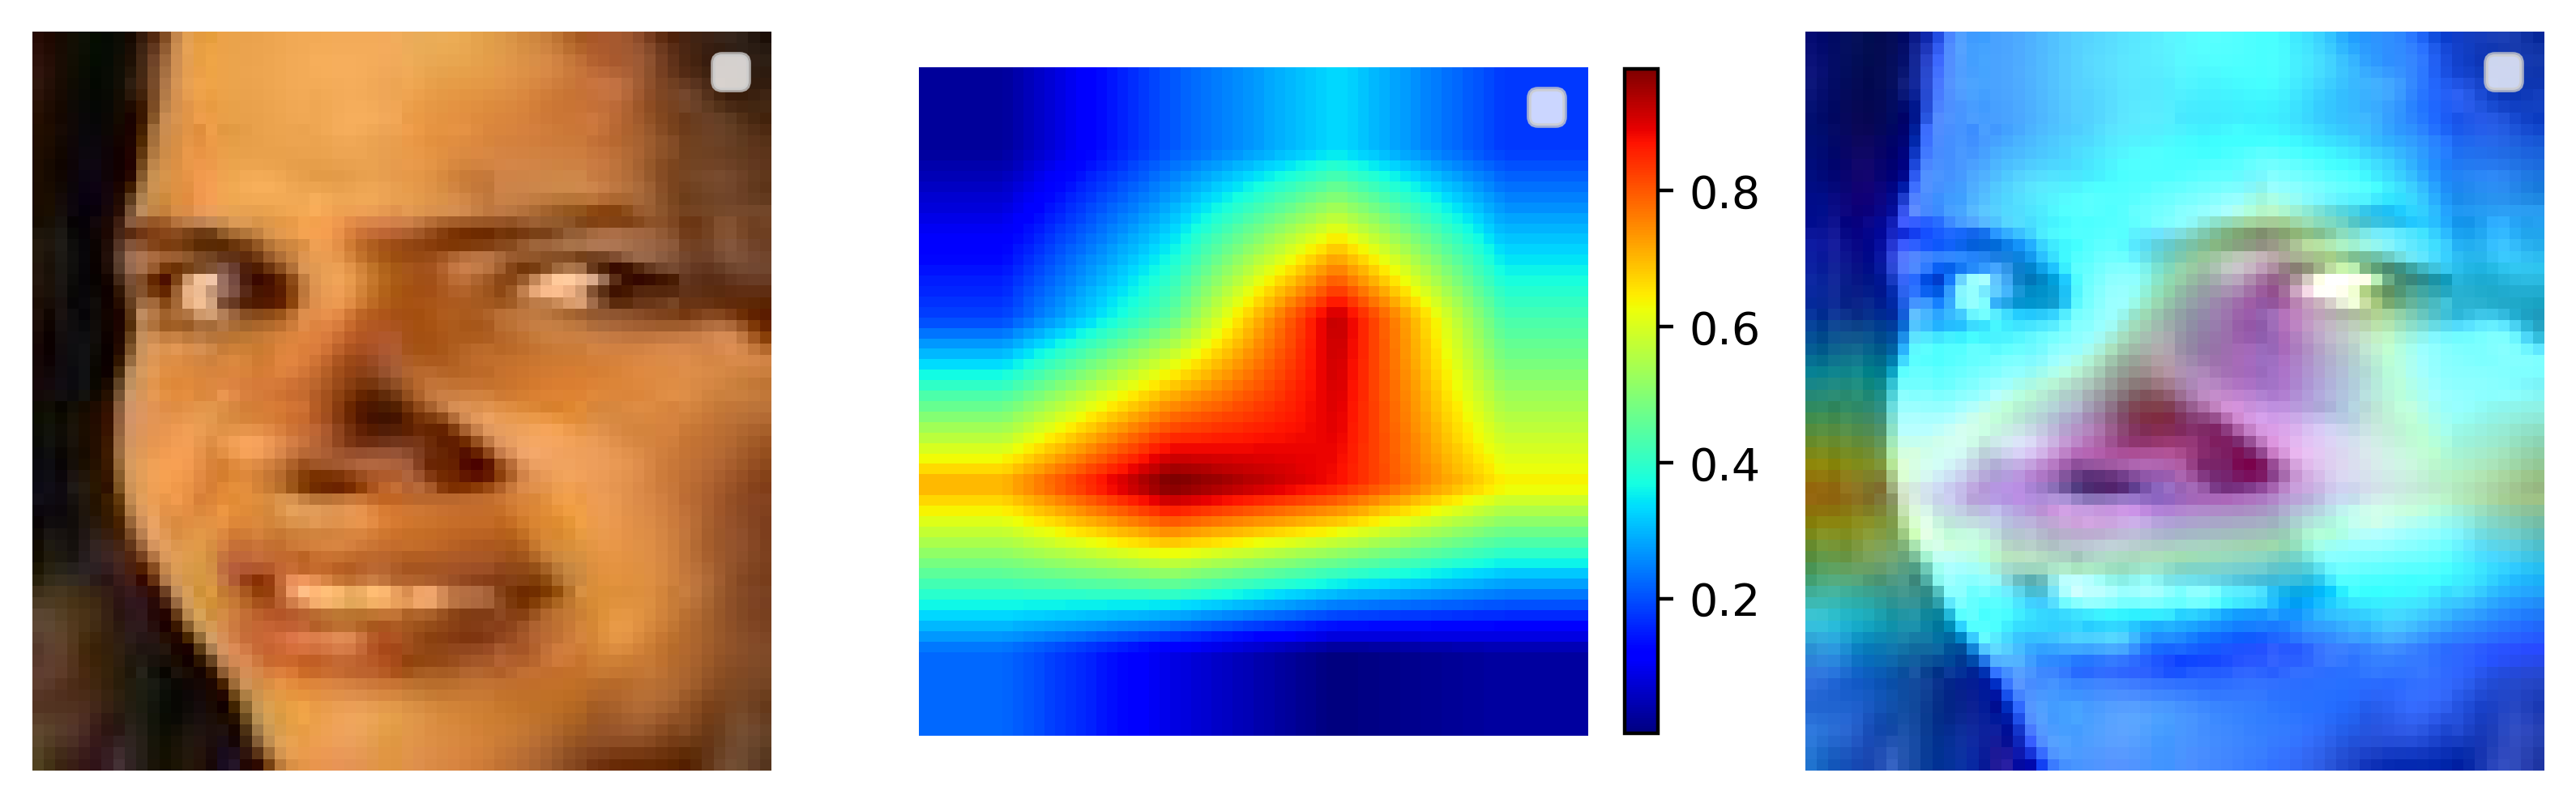
\includegraphics[width=\linewidth]{xai_disgust.png}
    \caption{Disgust.}
    \label{fig:xai5}
  \end{subfigure}
  \hfill
  \begin{subfigure}{0.3\linewidth}
    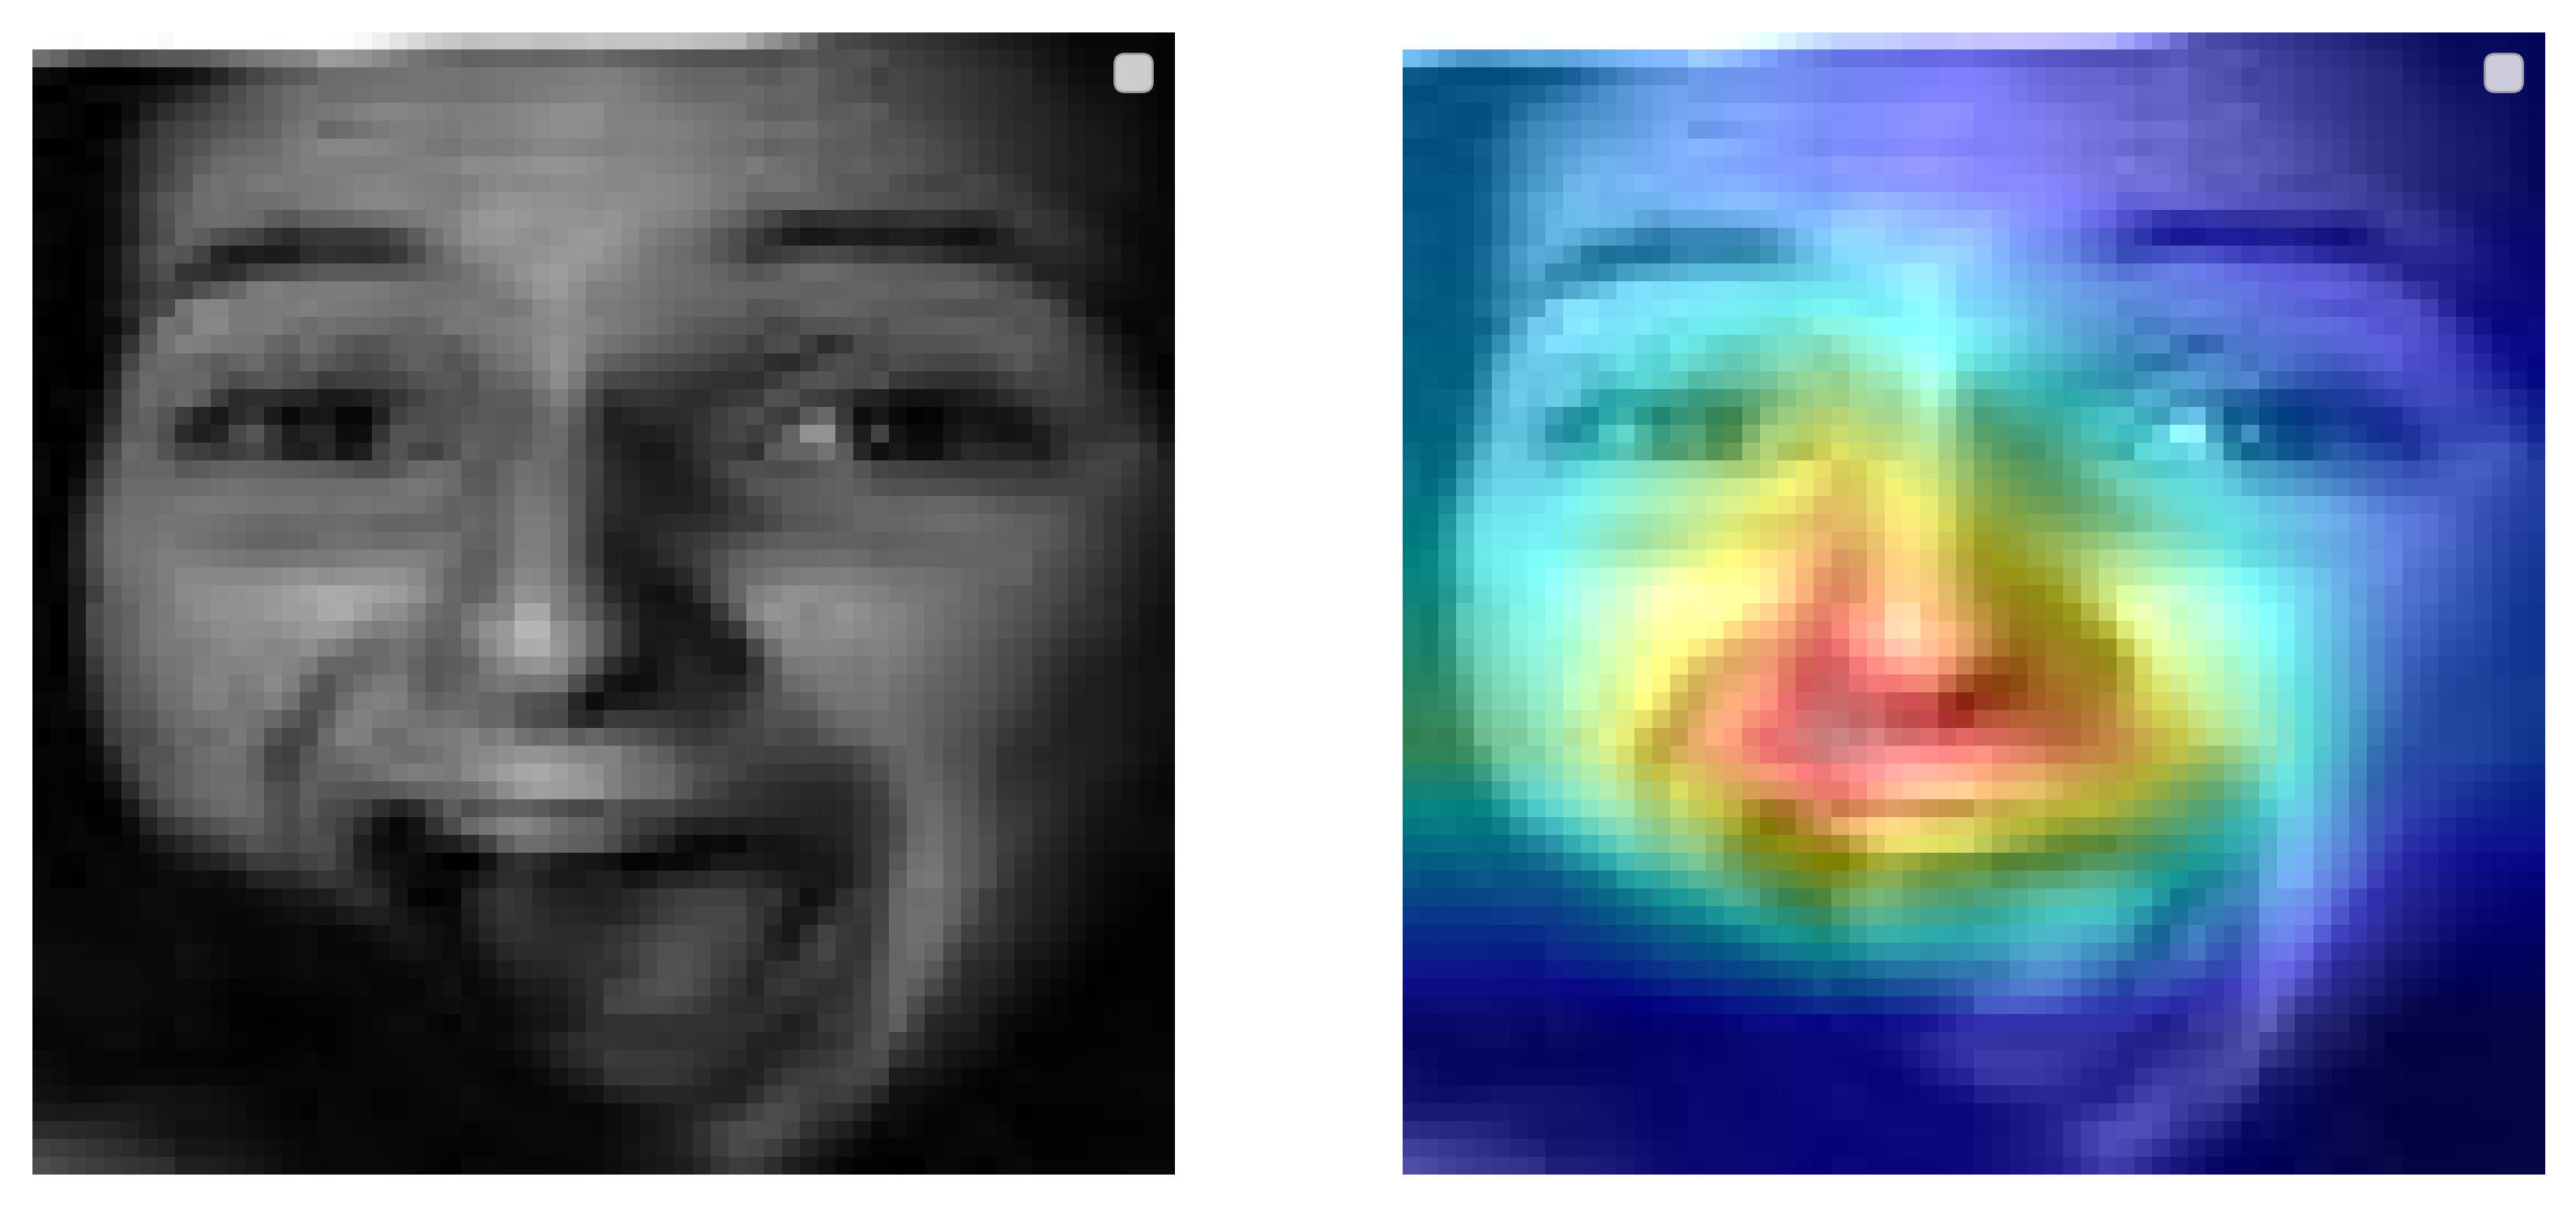
\includegraphics[width=\linewidth]{xai_fear.png}
    \caption{Fear.}
    \label{fig:xai6}
  \end{subfigure}
  % \hfill
  % \begin{subfigure}{0.15\linewidth}
  %   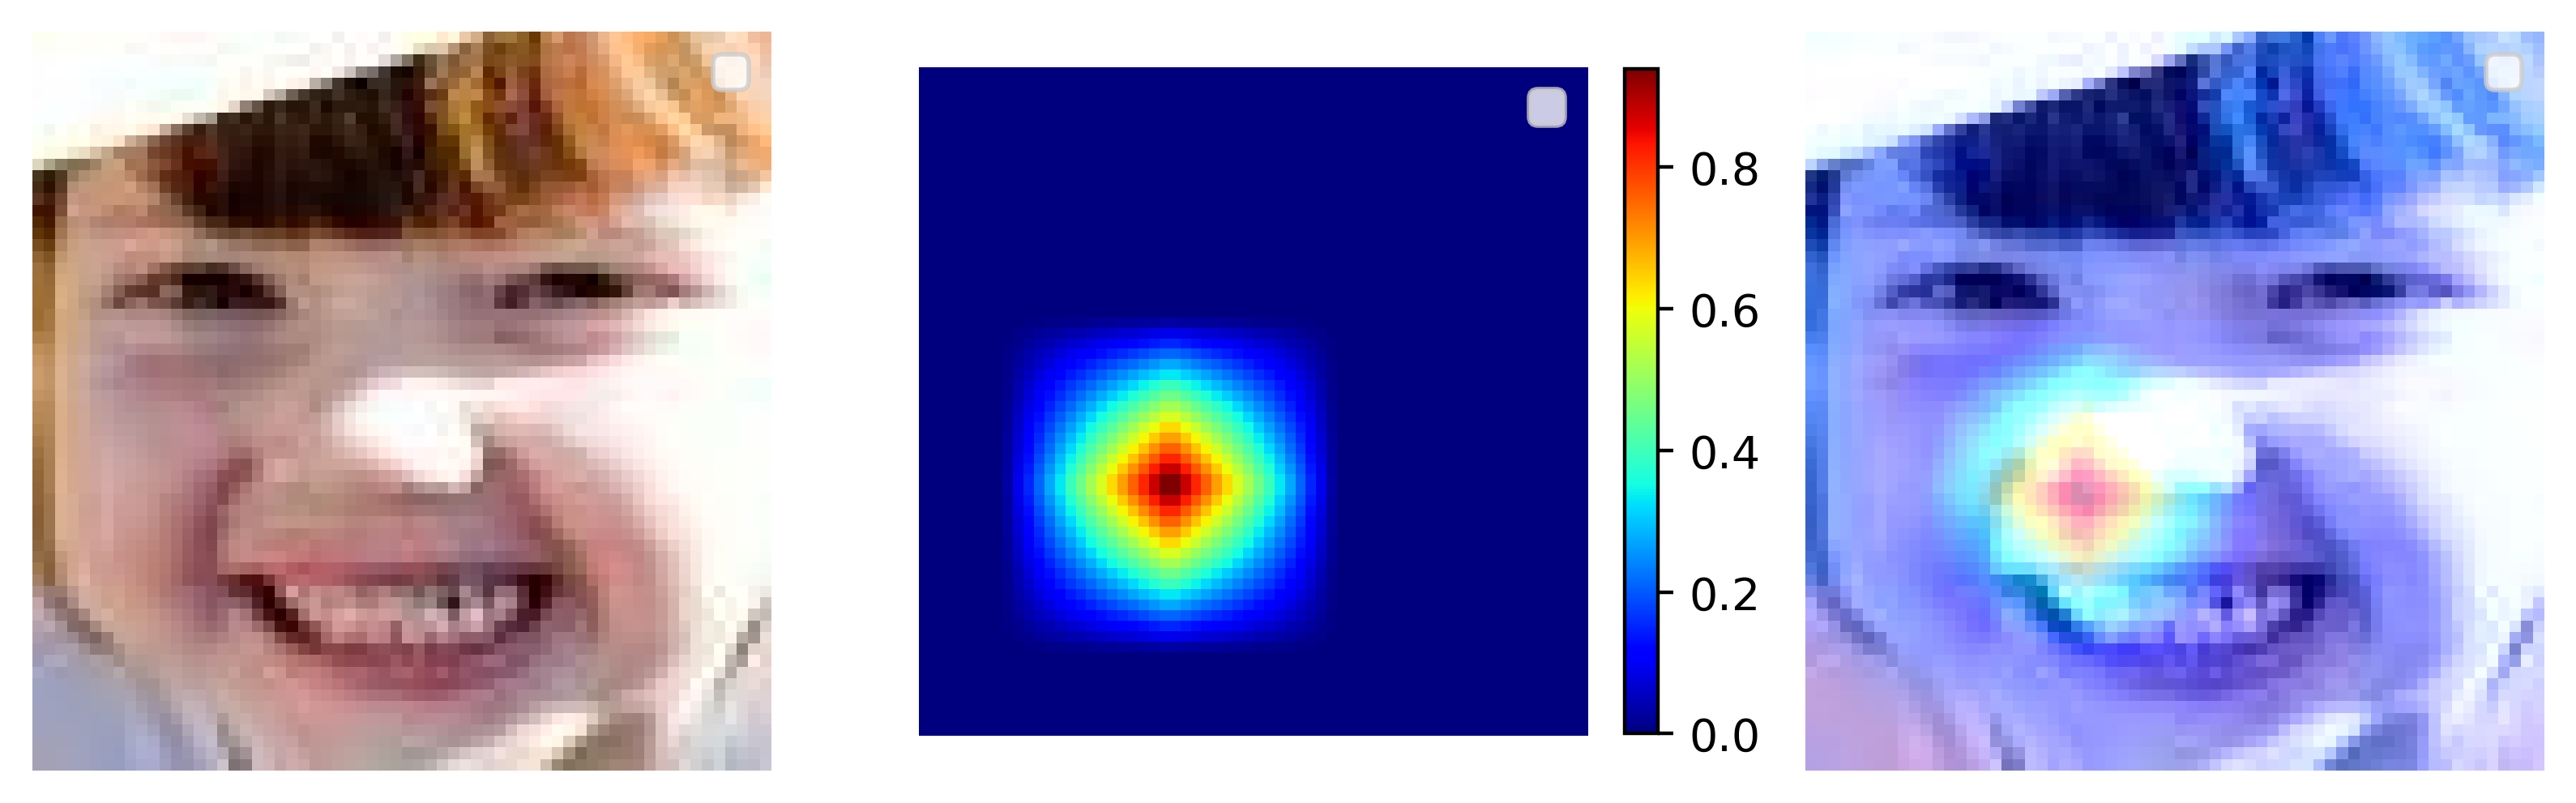
\includegraphics[width=\linewidth]{xai_happiness.png}
  %   \caption{Happiness.}
  %   \label{fig:xai7}
  % \end{subfigure}
  % \hfill
  % \begin{subfigure}{0.15\linewidth}
  %   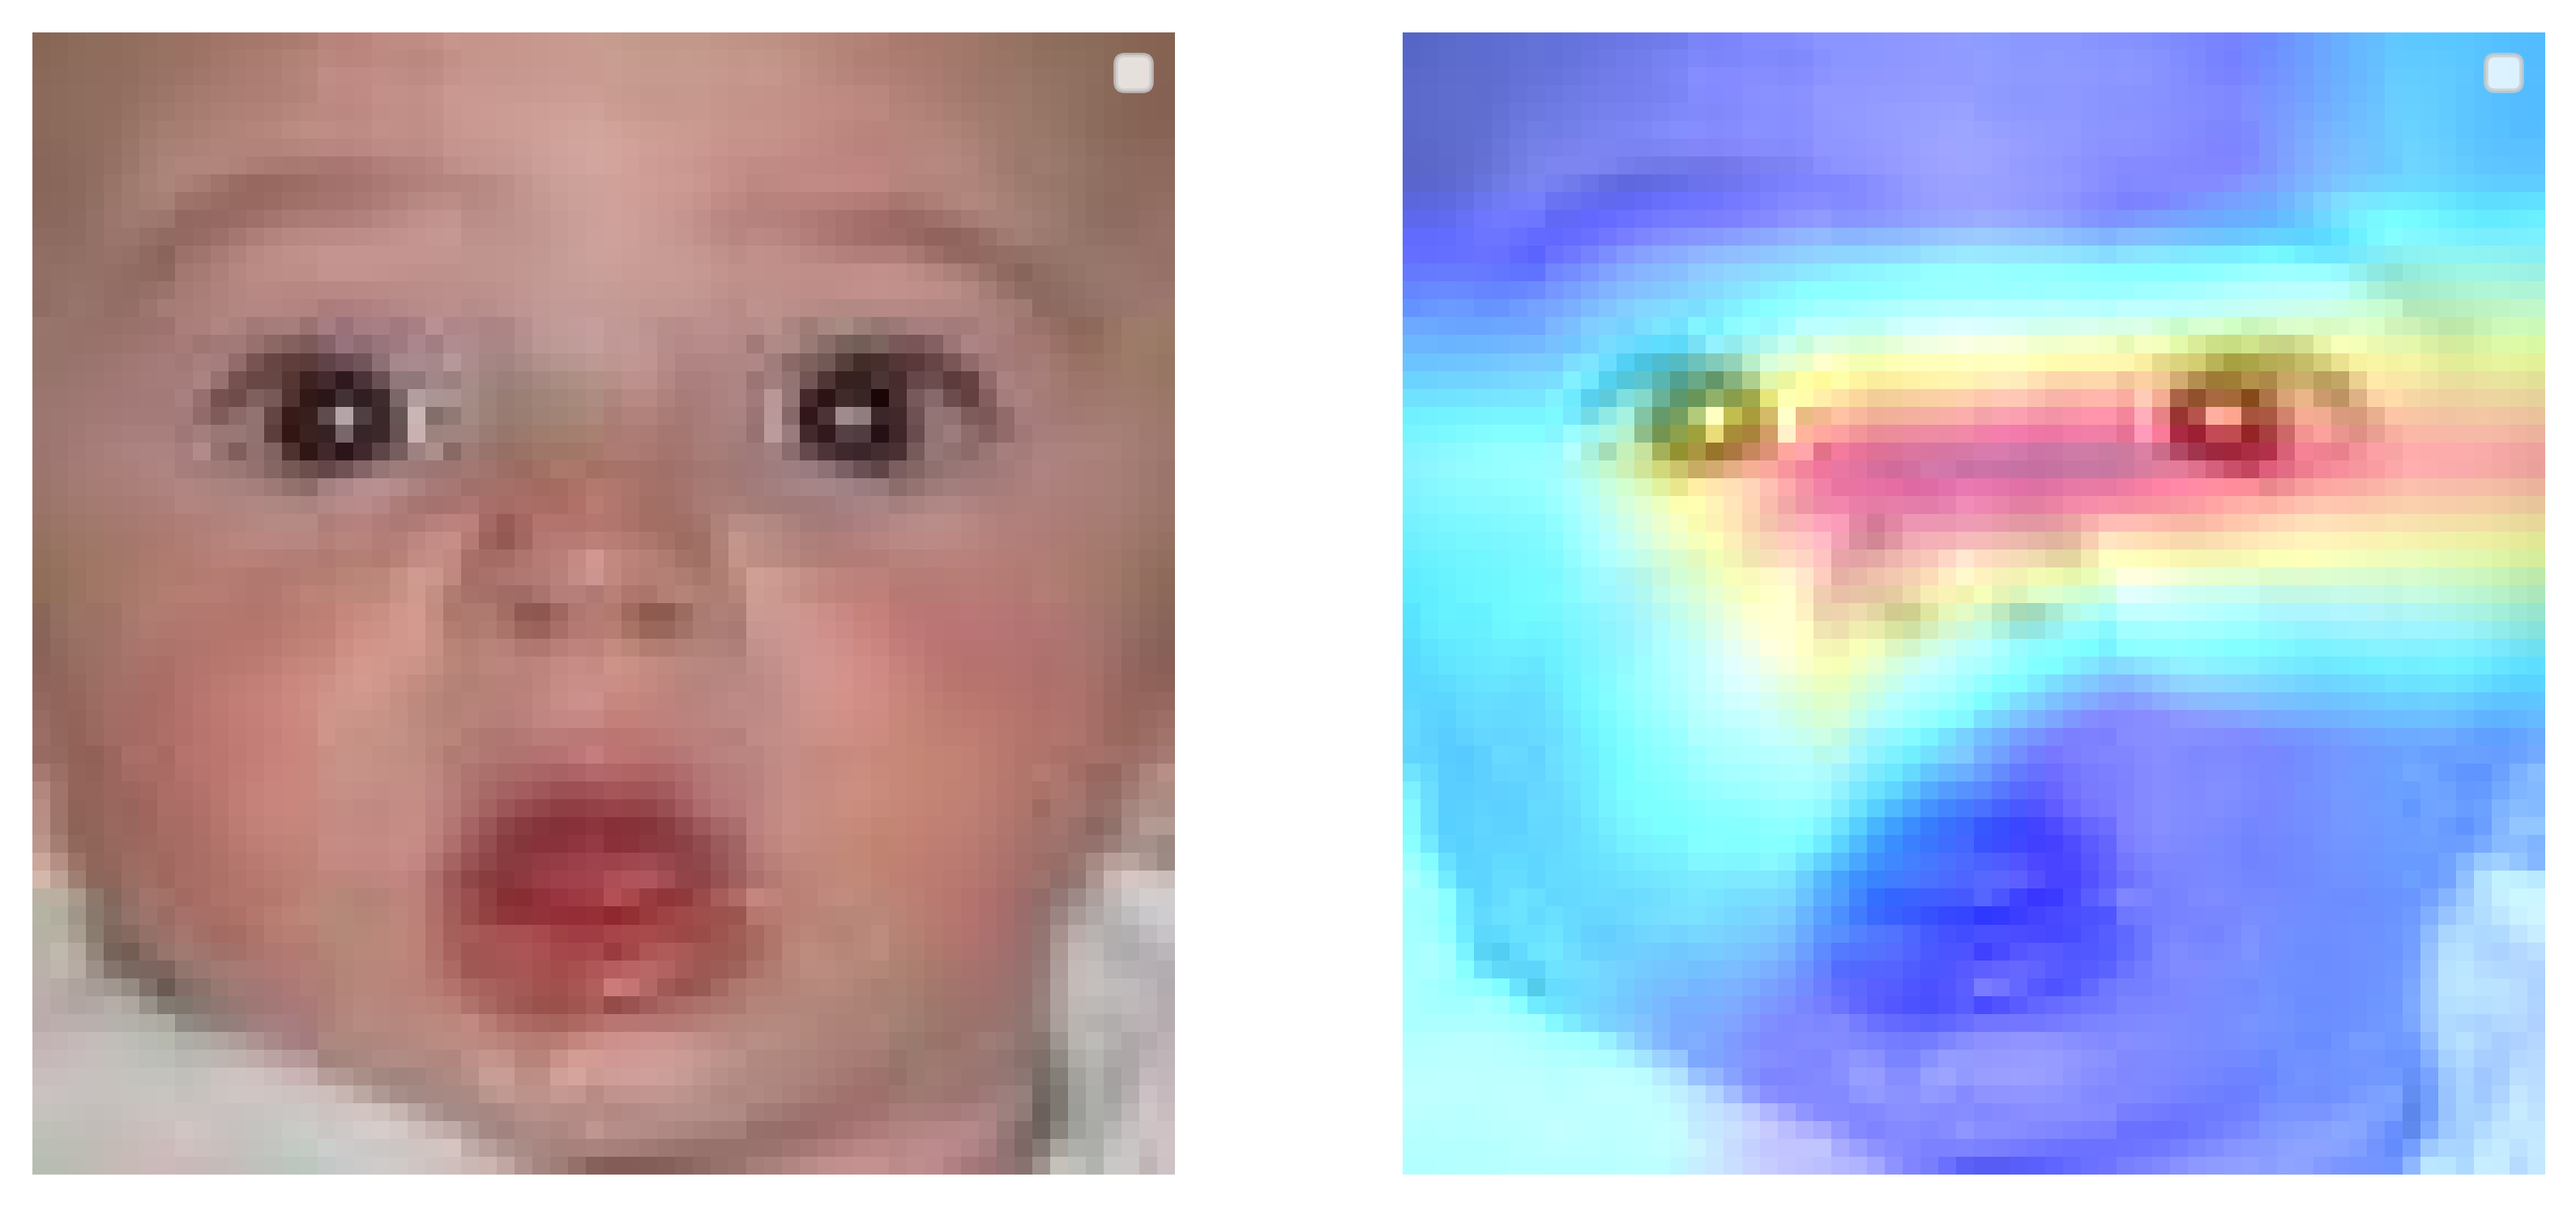
\includegraphics[width=\linewidth]{xai_surprise_.png}
  %   \caption{Surprise.}
  %   \label{fig:xai8}
  % \end{subfigure}
  % \hfill
  % \begin{subfigure}{0.15\linewidth}
  %   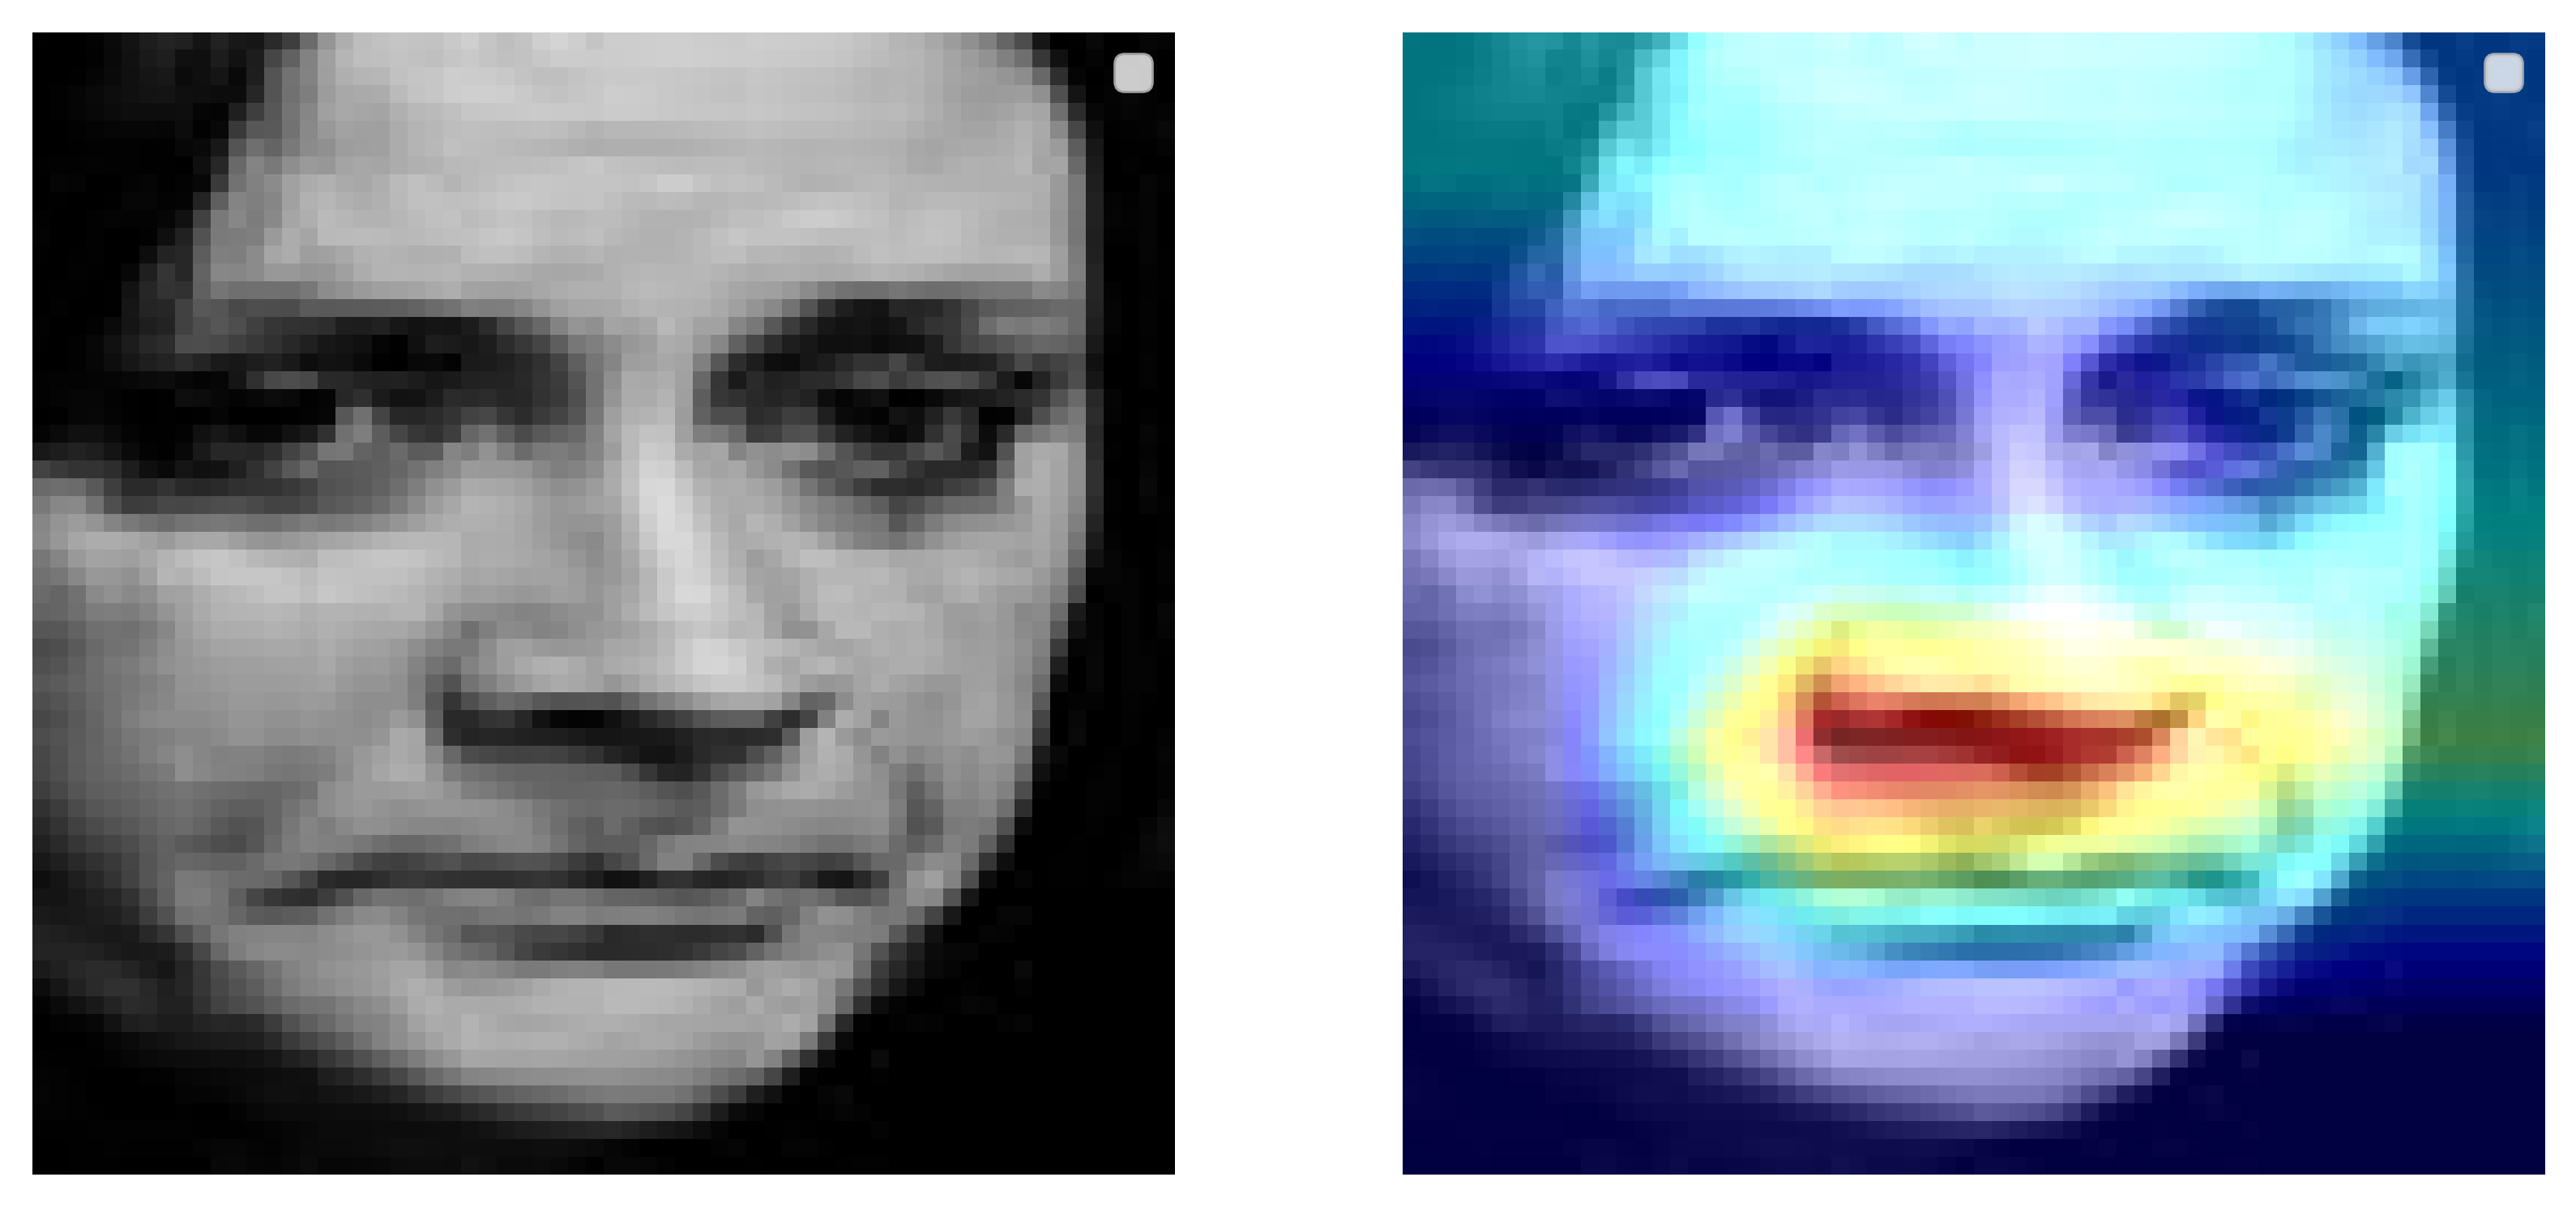
\includegraphics[width=\linewidth]{xai_sadness.png}
  %   \caption{Sadness.}
  %   \label{fig:xai9}
  % \end{subfigure}
  % \hfill
  % \begin{subfigure}{0.15\linewidth}
  %   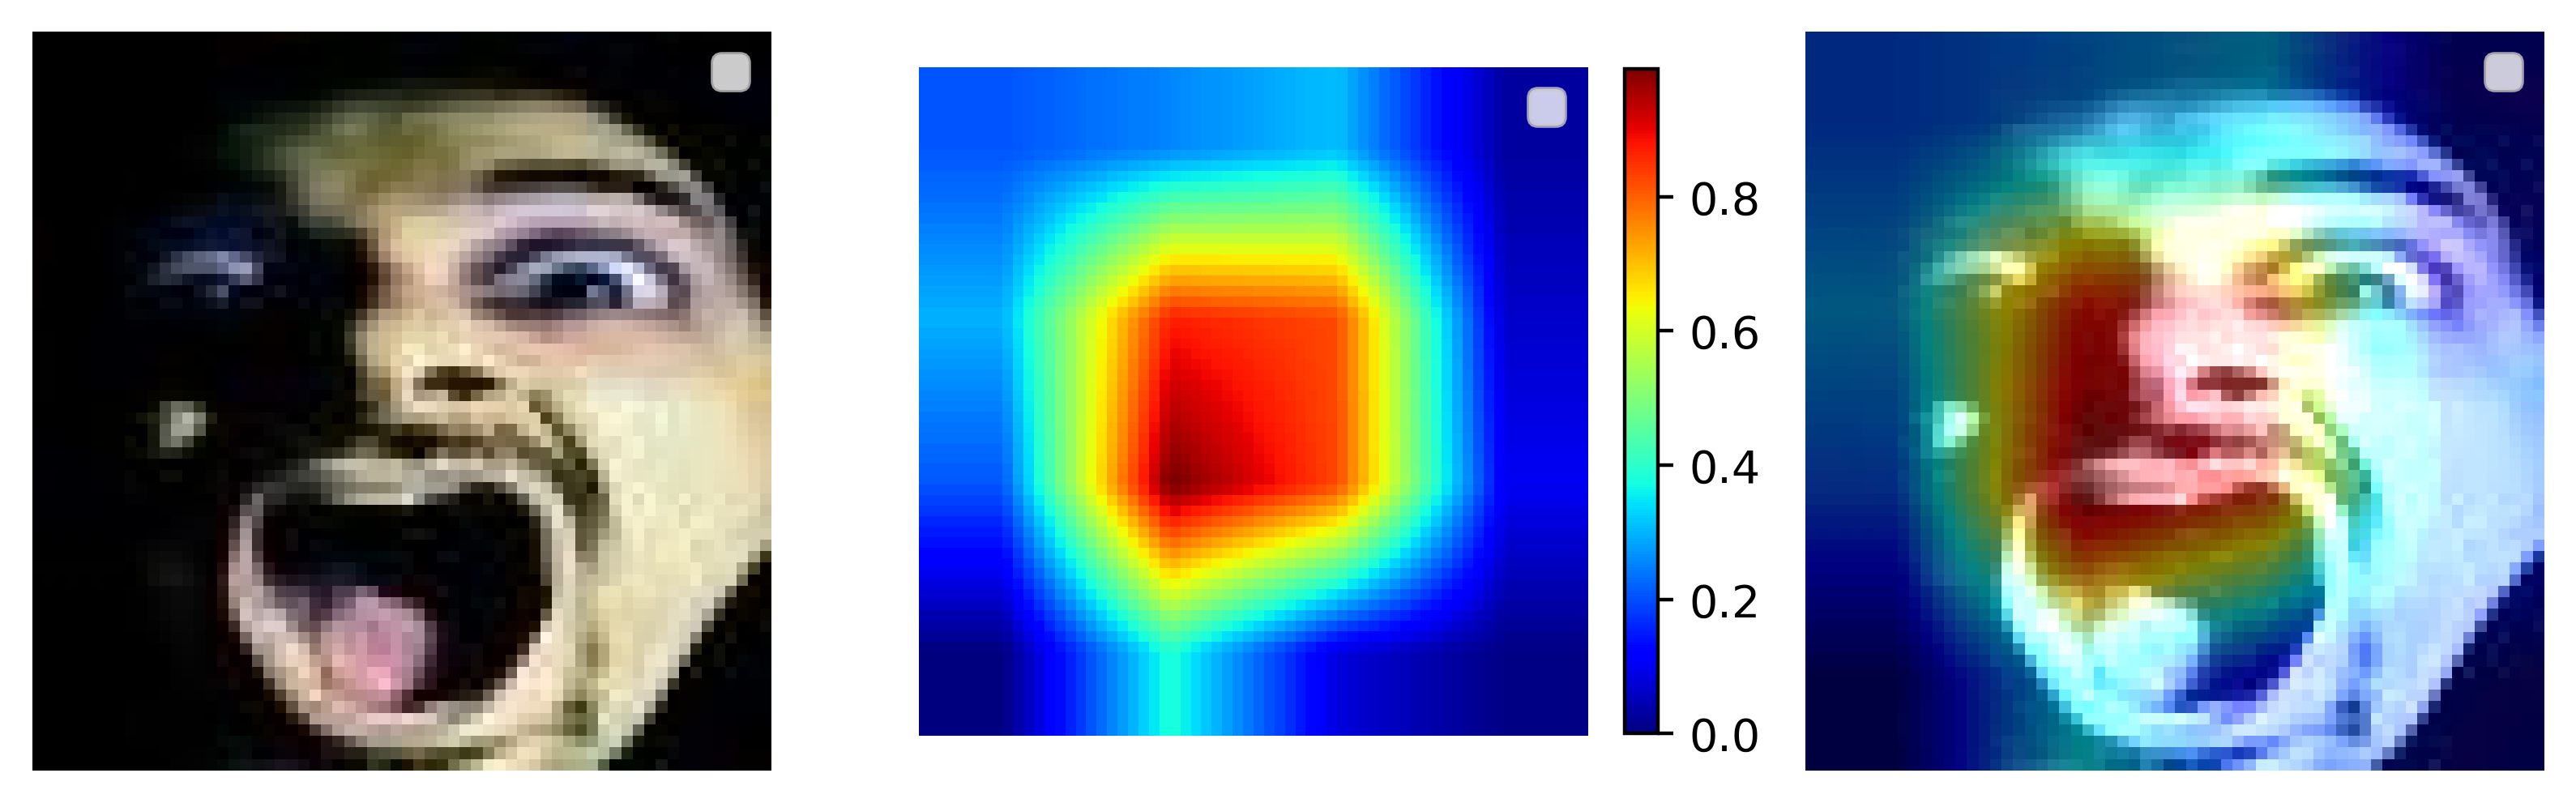
\includegraphics[width=\linewidth]{xai_anger_.png}
  %   \caption{Anger.}
  %   \label{fig:xai10}
  % \end{subfigure}
  % \hfill
  % \begin{subfigure}{0.15\linewidth}
  %   
\includegraphics[width=\linewidth]{xai_disgust_.png}
  %   \caption{Disgust.}
  %   \label{fig:xai11}
  % \end{subfigure}
  % \hfill
  % \begin{subfigure}{0.15\linewidth}
  %   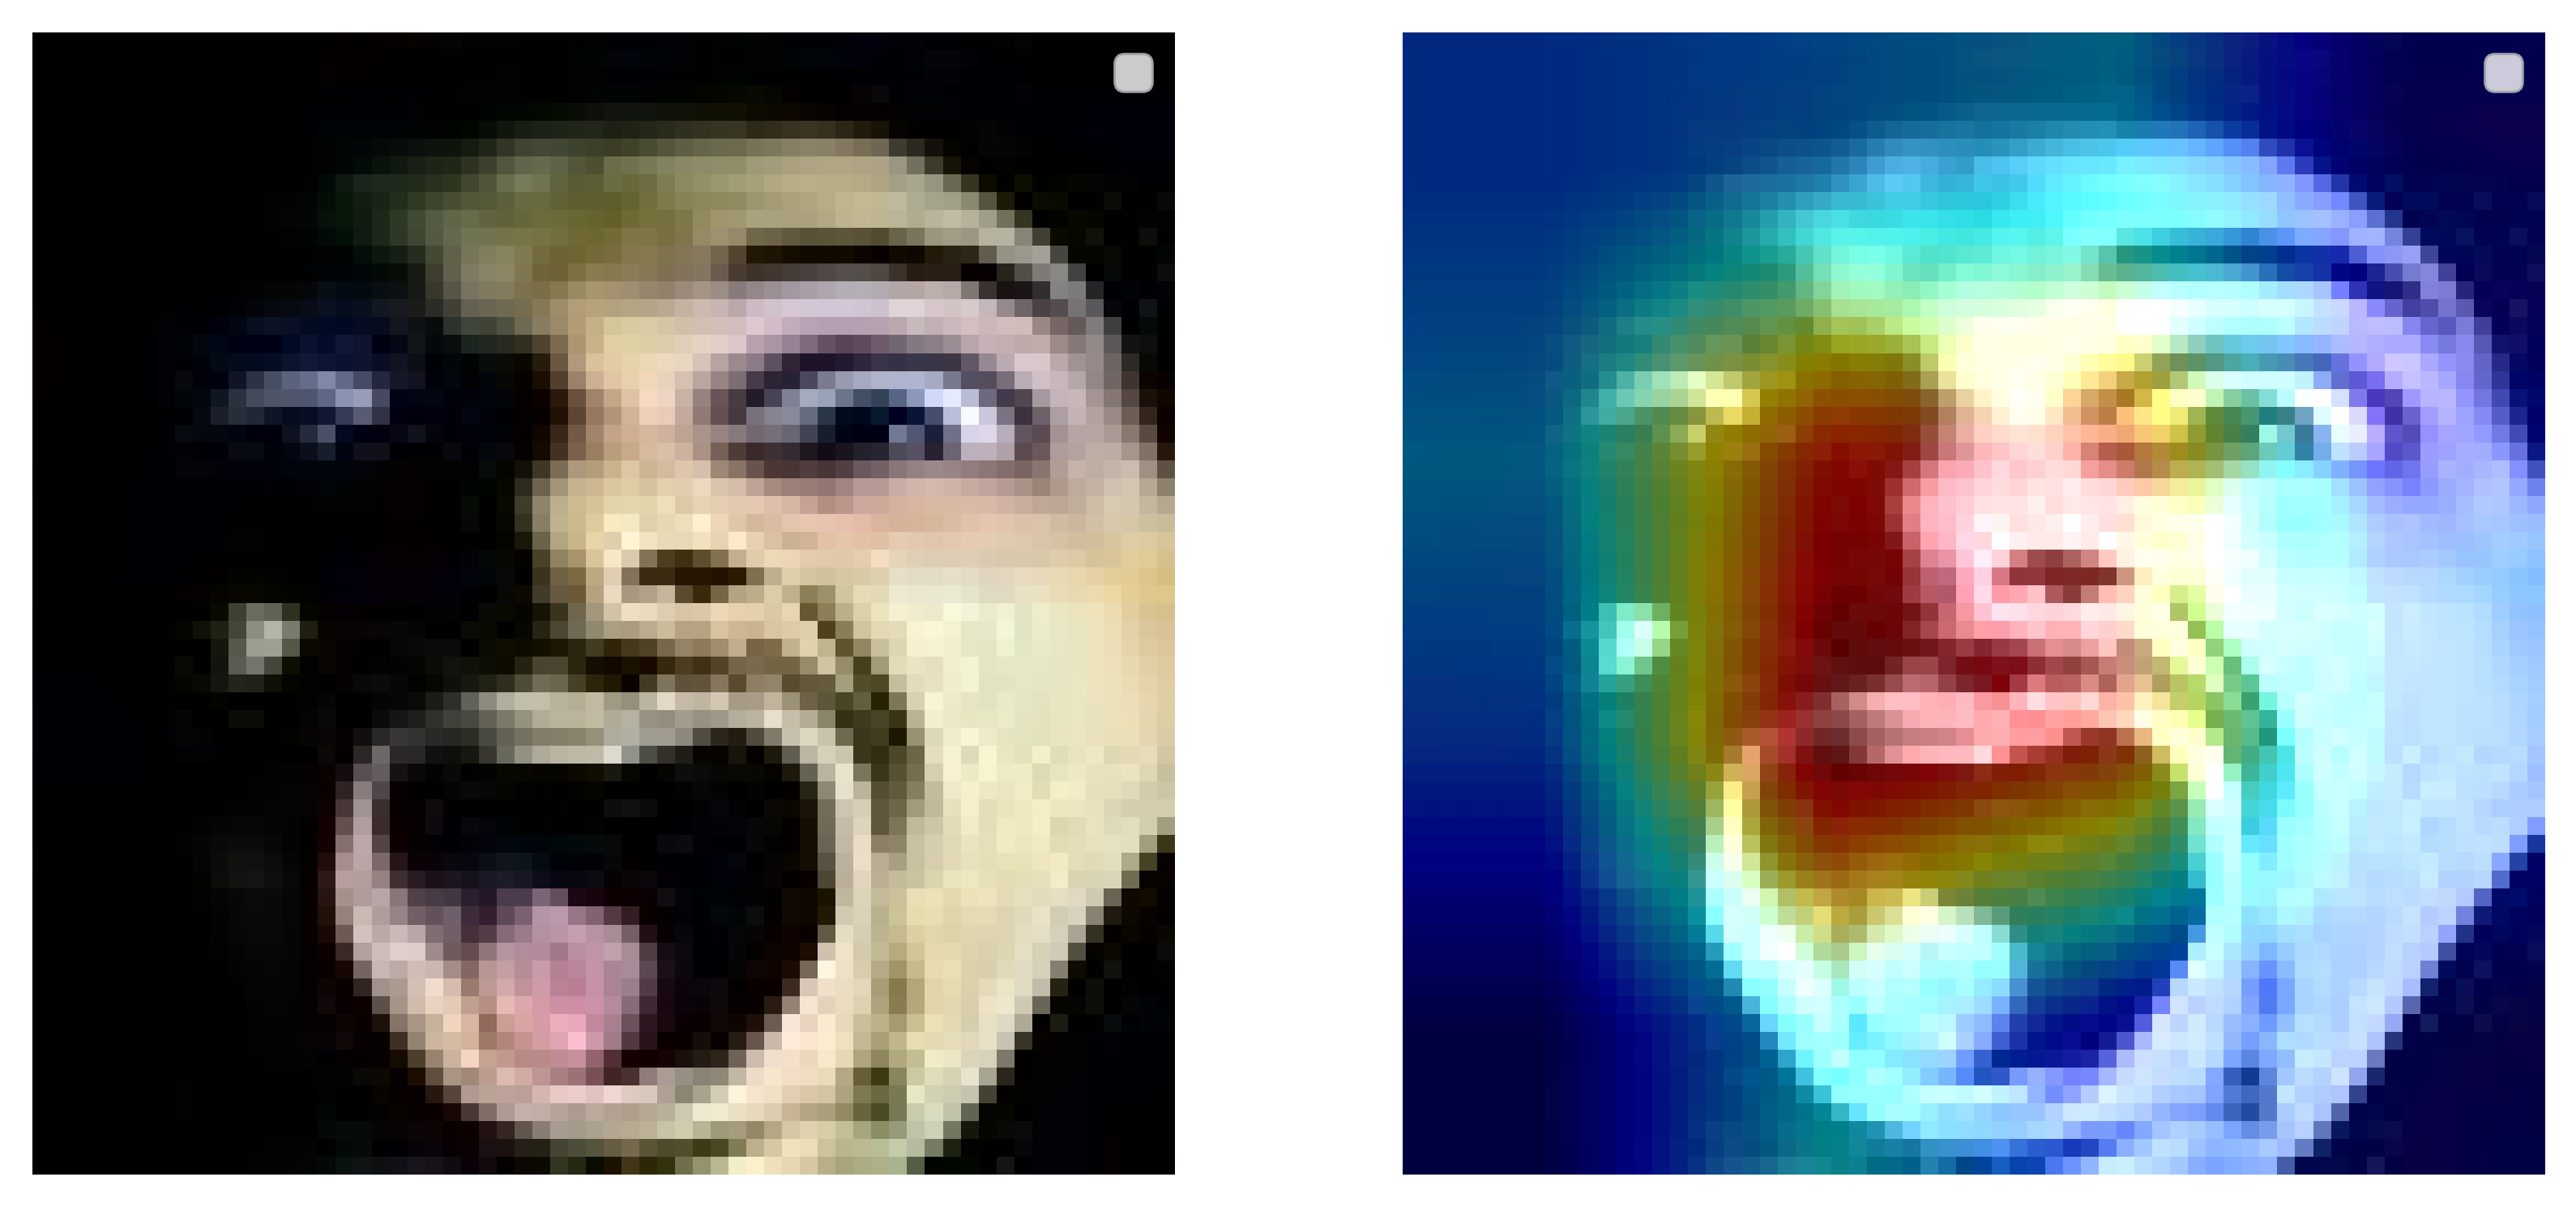
\includegraphics[width=\linewidth]{xai_fear_.png}
  %   \caption{Fear.}
  %   \label{fig:xai12}
  % \end{subfigure}
  \caption{Overview of explainable AI with all six facial emotional classes on the validation set.}
  \label{fig:xai}
\end{figure}

\paragraph{Heatmap Overlayed Grad-CAM.}
In our case, we leverage the last (i.e., fifth) convolutional layer of our model to generate the CAM heatmap. 
The \textit{global average pooling} (GAP) layer, 
which computes the average value of each feature map to obtain a spatial average of feature maps, 
is used to obtain a spatial average of the feature maps. 

\paragraph{Overlay evaluated emotions.} % TODO Leah
The GiMeFive classifications of every frame are plotted in percentage next to the saliency map (heatmap).
On top of the saliency map the main emotion, extracted from every fifth frame, is written, so it is easier for our eyes to adapt.

\begin{figure*}[ht]
  \centering
  \begin{subfigure}{0.24\linewidth}
    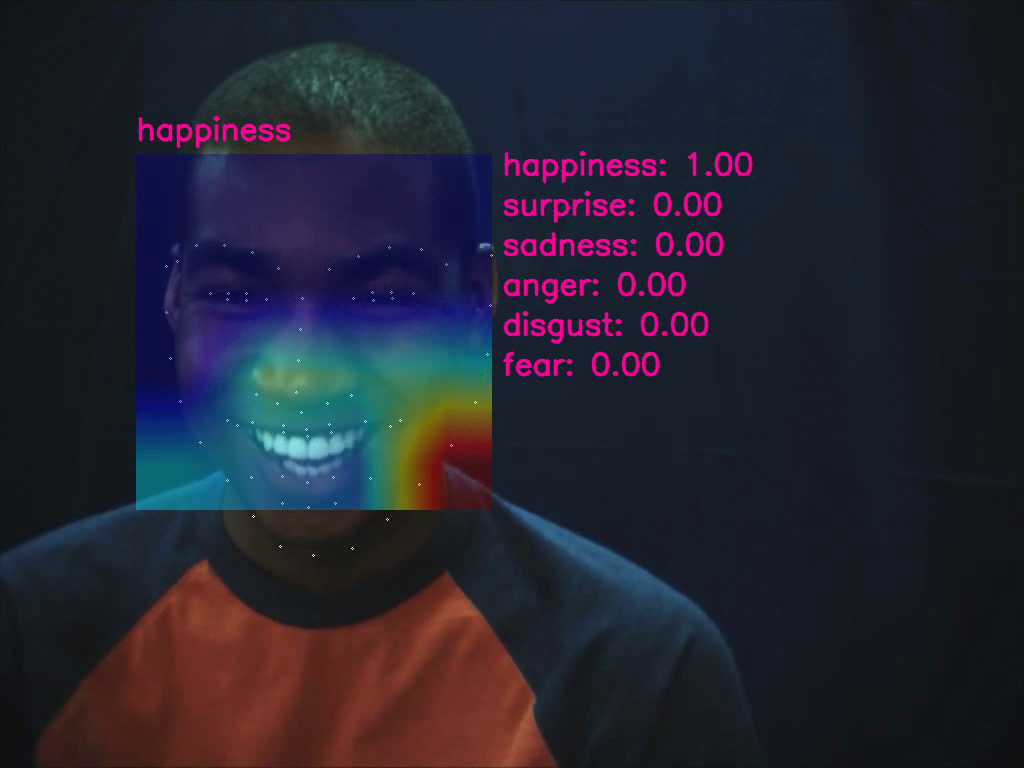
\includegraphics[width=\linewidth]{GiMeFive01.png}
    \caption{Happiness.}
    \label{fig:v1}
  \end{subfigure}
  \hfill
  \begin{subfigure}{0.24\linewidth}
    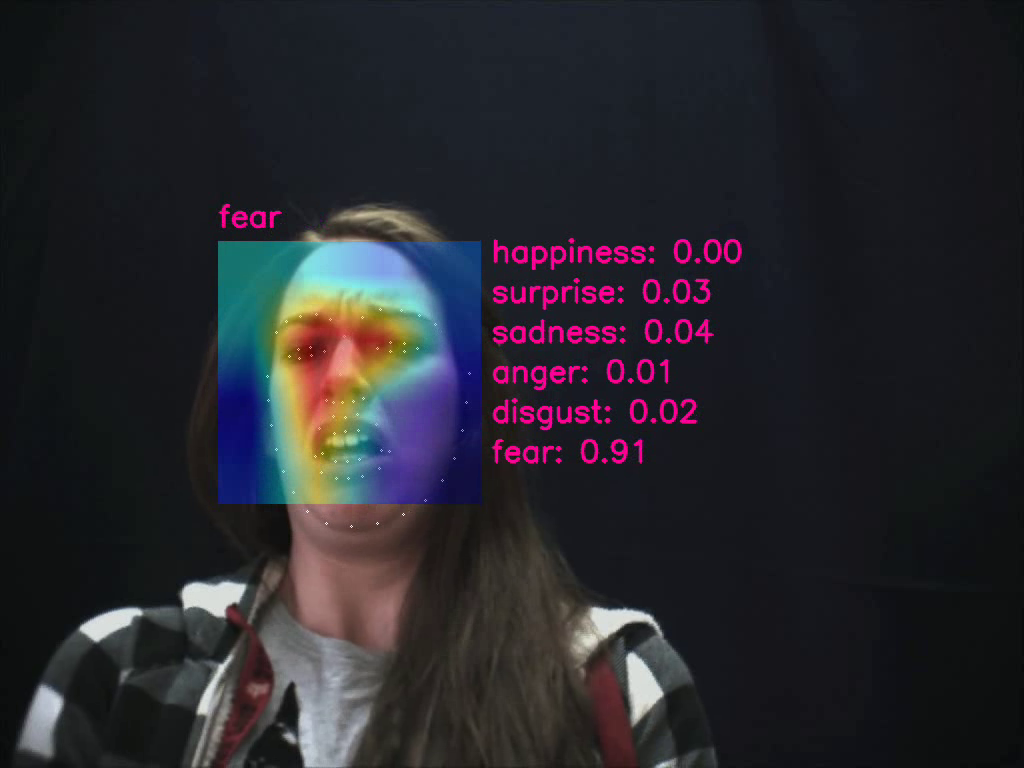
\includegraphics[width=\linewidth]{GiMeFive02.png}
    \caption{Fear.}
    \label{fig:v2}
  \end{subfigure}
  \hfill
  \begin{subfigure}{0.24\linewidth}
    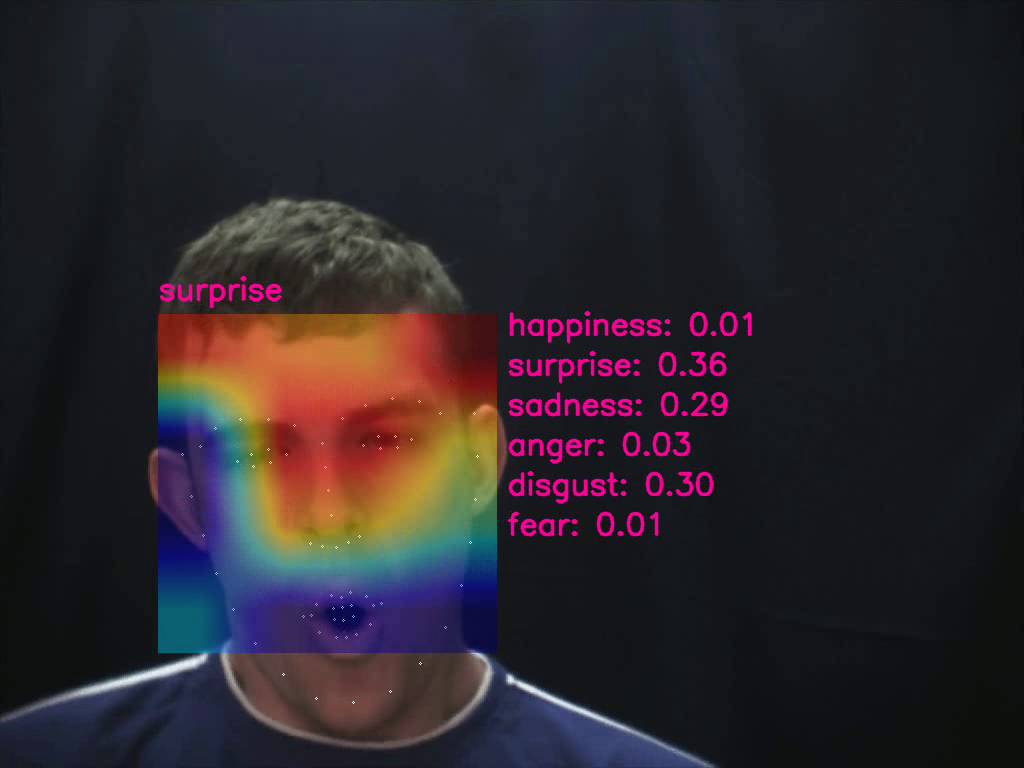
\includegraphics[width=\linewidth]{GiMeFive03.png}
    \caption{Surprise.}
    \label{fig:v3}
  \end{subfigure}
  \hfill
  \begin{subfigure}{0.24\linewidth}
    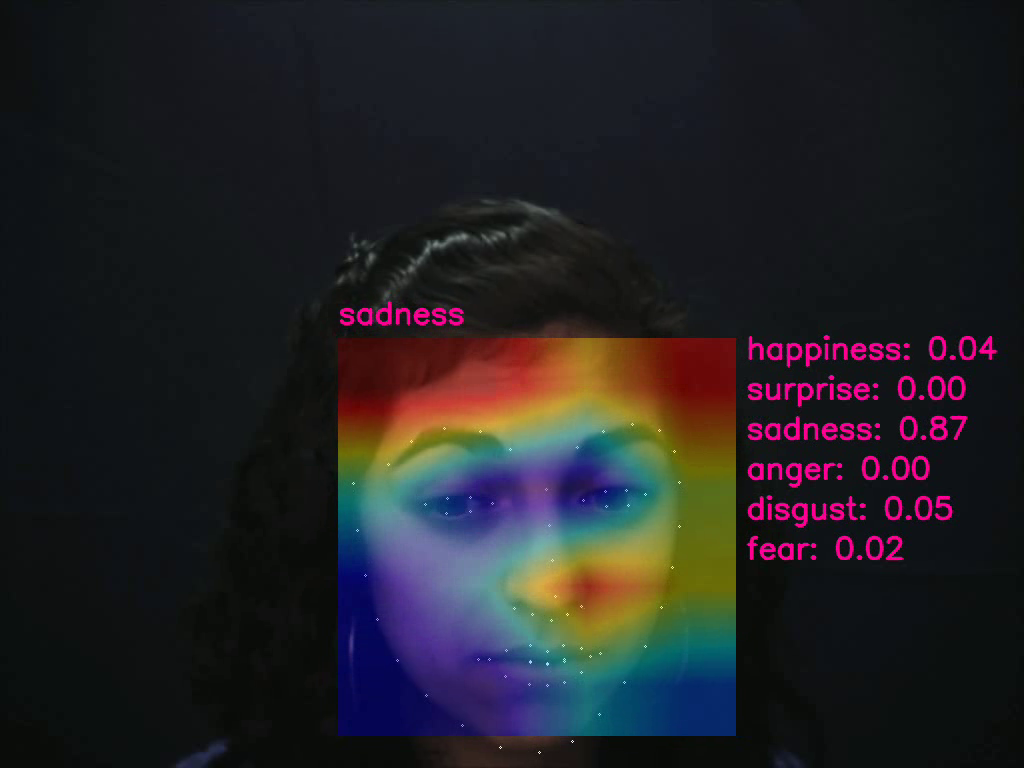
\includegraphics[width=\linewidth]{GiMeFive04.png}
    \caption{Sadness.}
    \label{fig:v4}
  \end{subfigure}
  \hfill
  \caption{Overview of XAI with grad-CAM and landmarks on DISFA dataset.}
  \label{fig:video}
\end{figure*}

\paragraph{Landmarks.}
To plot Landmarks on each video frame, we implemented the pretrained dlib shape predictor 
\texttt{dlib shape predictor}, % worked ;P
\texttt{shape predictor 68 face landmarks.dat}, 
constructed using the classic Histogram of Oriented Gradients feature (HOG)~\cite{1467360} combined with a linear classifier, 
an image pyramid, and sliding window detection scheme.~\cite{dlib_site}
The pose estimator was created using the implementation dlib from \citet{6909637}.

With this pertained model, 68 numbered Landmarks assist emotion analysis, 
and facial expression tracking, to understand and interpret facial features.
We implement using the libraries such as Dlib~\footnote{~\url{http://dlib.net/}}. % Für dlib
Again, \Cref{{fig:v1}} happiness the easy to detection in principle 


% TODO (Jiawen)

\section{Optimization Strategies}
\label{sec:optim}

To further understand and enhance the performance of the model during training, 
% we focus on the following tasks, 
% i.e., data augmentation (see \Cref{sec:optim:aug}), 
% CAM (see \Cref{sec:optim:cam}), and Grad-CAM (see \Cref{sec:optim:gcam}). 
%~\footnote{\url{https://github.com/maelfabien/Multimodal-Emotion-Recognition}}. 

\subsection{Data Augmentation}
\label{sec:optim:aug}

For augmentation we determined \texttt{RandomHorizontalFlip}, \texttt{RandomRotation}, 
\texttt{RandomCrop}, and \texttt{RandomErasing} at the very begining. 
In deep learning and AI, 
augmentation~\cite{augment} stands as a transformative technique, 
empowering algorithms to learn from and adapt to a wider range of data. 
By introducing subtle modifications to existing data points, 
augmentation effectively expands the dataset, 
enabling models to generalize better and achieve enhanced performance. 
As models encounter slightly altered versions of familiar data, 
they are forced to make more nuanced and robust predictions. 
With this process, we aim to prevent overfitting, which is a common pitfall in machine learning. 
Additionally, we guide the training process to enhance the recognition and handling of real-world variations.
Meanwhile, we create various replications of existing photos by randomly altering different properties such as size, brightness, color channels, or perspectives.

\subsection{Hyperparameter Tuning}
\label{sec:optim:tuning}

\begin{table}[ht]
  \centering
  \begin{tabular}{@{}lc@{}}
    \toprule
    \textsc{Hyperparameter} & \textsc{Value} \\
    \midrule
    Learning rate & $ \{\num{1e-2}, \num{1e-3}, \num{1e-4} \} $ \\
    Batch size & \{8, 16, 32, 64\} \\
    Dropout rate & \{0.2, 0.5\} \\
    Convolution depth & \{4, 5, 6\} \\
    Fully connected depth & \{1, 2, 3\} \\
    Batch normalization & \{\texttt{True}, \texttt{False}\} \\
    Pooling & \{\texttt{max}, \texttt{adaptive avg}\} \\
    Optimizer & \{\texttt{Adam}, \texttt{AdamW}, \texttt{SGD}\} \\
    Activation & \{ \texttt{relu}\} \\ % , \texttt{tanh}, \texttt{elu}, \texttt{gelu}
    Epoch & \{10, 20, 40, 80\} \\
    Early stopping & \{\texttt{True}, \texttt{False}\} \\
    Patience & \{5, 10, 15\} \\
    \bottomrule
  \end{tabular}
  \caption{Explored hyperparameter space for our models.}
  \label{tab:hyper}
\end{table}

In order to find the best hyperparameter configuration (see \Cref{tab:hyper} for details) of the model, 
we utilize the parameter grid from Sklearn.
% ~\footnote{\url{https://scikit-learn.org/stable/modules/generated/sklearn.model_selection.ParameterGrid.html}}.
Additionally, 
we increase the depth of the network by adding some convolutional layers to learn more complex features. 
To help the training of deeper networks more efficiently, 
we add the residual connections, 
as they allow gradients to flow through the network more easily, 
improving the training for deep architectures. 
Moreover, 
we add \textit{squeeze and excitation} (SE) blocks to apply channel-wise attention. 

\section{Conclusion and Discussion}
\label{sec:conclusion}

\paragraph{Limitations.}

\newpage
% \clearpage
